\chapter{The CMS Resistive Plate Chambers}\label{chap:rpc}
%================================================================

This chapter will discuss about on the CMS RPC system, where the author was able to work. A brief history of gaseous detectors will be presented, with focus on the RPC detector. The CMS RPC project will be introduced and the work my contributions will be presented.

\section{Brief history of gaseous detectors}

The first gaseous detector was introduced by E. Rutherford and H. Geiger in 1908 \cite{rutherford1908electrical}. The device consisted in a thin wire, the anode, coaxial to a cylindrical cathode filled with gas. When a ionizing particle passed through the gas, it ionized the gas particles. By applying a difference of potential to the device, the released electrons accelerate to the anode and inelastic collisions with other molecules multiplying the effect of the ionization in the so-called avalanche process, which was studied by John Sealy Townsend, between 1897 to 1901 \cite{peskov2018resistive}. An illustration of the avalanche formation in gaseous detectors is shown in Fig. \ref{fig:avalanche}. This kind of detector is still used up to today, mainly on radiation detection and monitoring.

\begin{figure}[!htm]{15cm}
\caption{Avalanche formation in gaseous detectors}%
\label{fig:avalanche}
\fbox{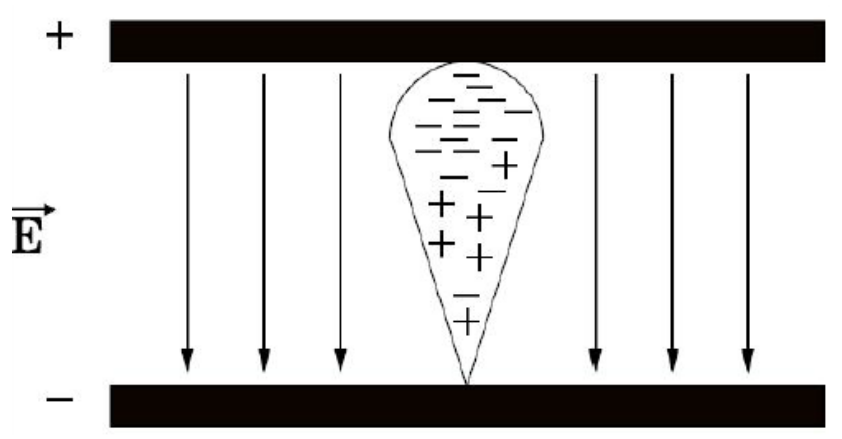
\includegraphics[width=0.5\hsize]{figures/avalanche_formation.png}}
\legend{The formation of a avalanche in gaseous detectors. The ionised electrons drift towards the anode because of the external electric field. As they accelerate, new electrons-ion pairs are formed multiplying the initial ionisation. The drop-like shape of the avalanche is caused by the difference in the drift velocity of electrons and ions.}
\source{\cite{Shopova:2626243}}
\end{figure}

This device operation depends on the applied voltage as shown Fig. \ref{fig:gaseous_curve}. At lower electric field strength, the electron and ions drifts with no avalanche multiplication and the number of electron-ion pairs is independent of of the voltage, at the ionization chamber mode. At the proportional mode the avalanche process occurs for each ionization, so that the number of electron-ion pairs is proportional to the energy deposited by the ionizing particle in the detector. Finally, at even higher voltage, in the Geiger-Müller counter region, there is emission of UV photons creating multiple avalanches along the anode wire \cite{o1961detection}. Also, at higher voltage levels the avalanches can increase into streamers, and even to sparks.

\begin{figure}[!htm]{15cm} 
\caption{Gaseous Counter Characteristic Curve}%
\label{fig:gaseous_curve}
\fbox{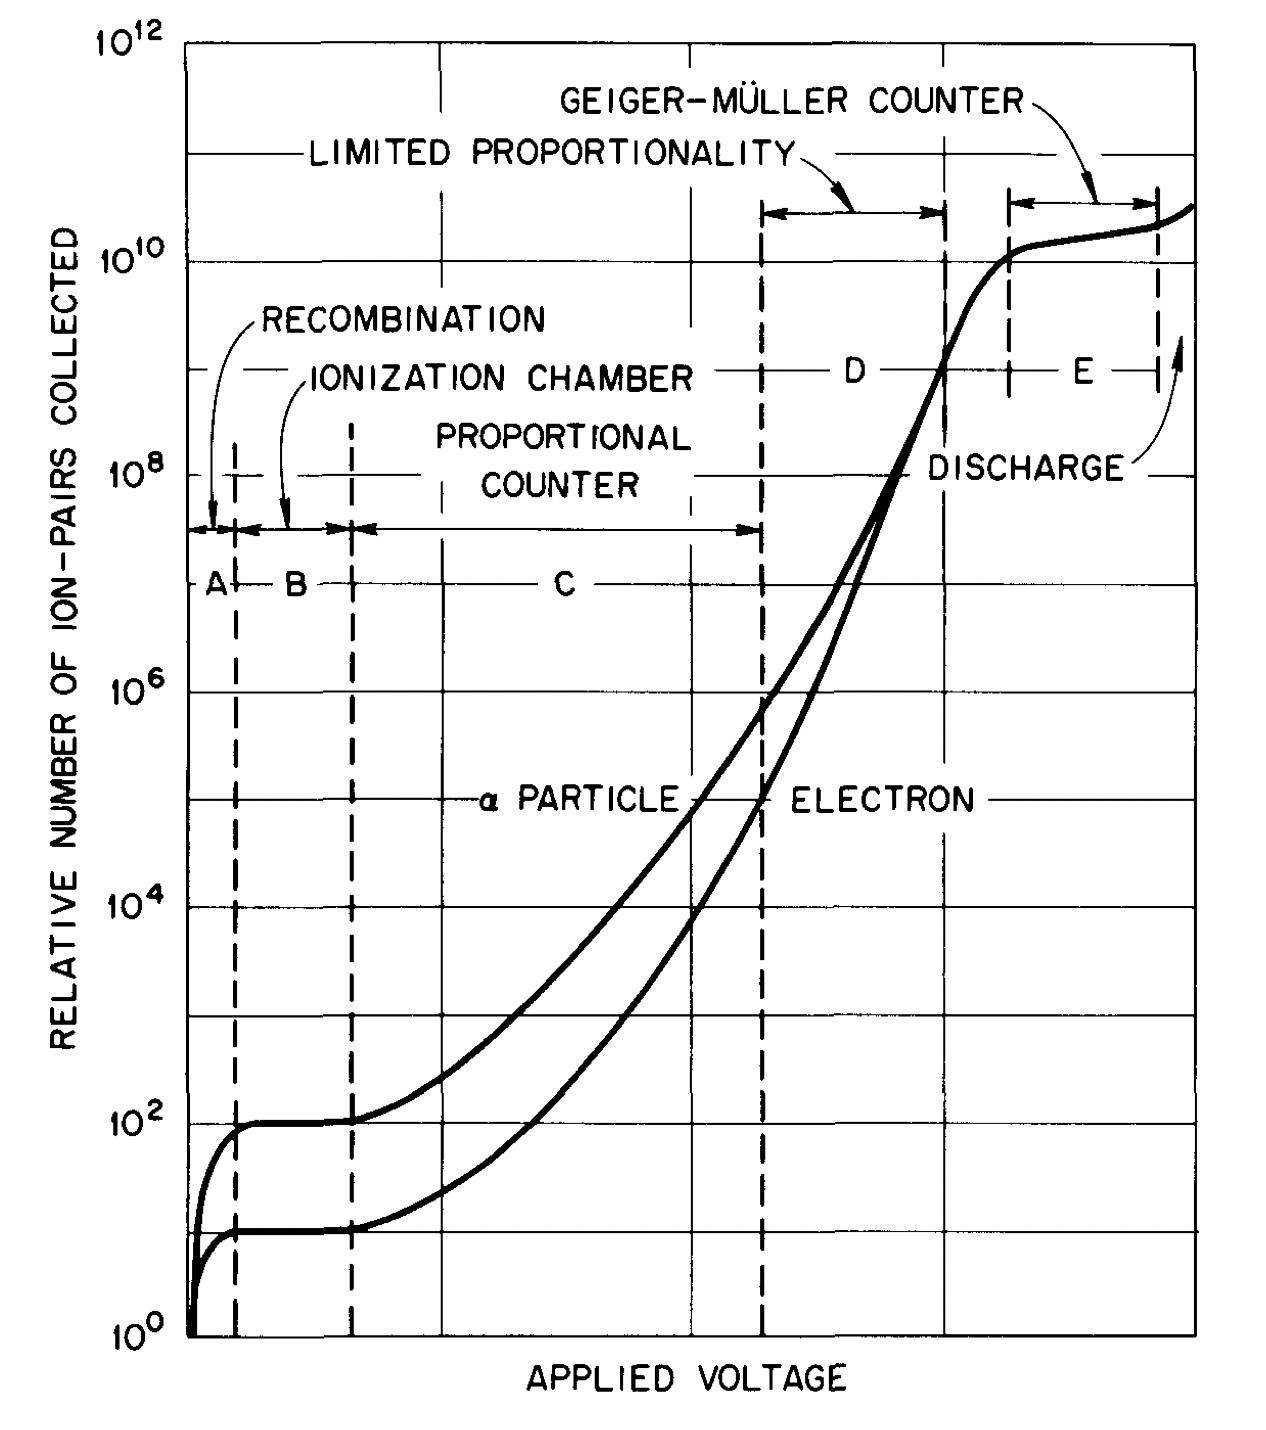
\includegraphics[width=0.5\hsize]{figures/gaseous_detector_curve.png}}
\legend{Curve of the relative number of ion pairs collected in a gaseous counter as a function of the applied voltage.}
\source{\cite{o1961detection}}
\end{figure}

But this devices are not suitable for the use in high-energy particle physics tracking. From the 1930s to the 1960s, the research was mainly done using cloud chambers as bubble chambers, which have excellent imaging capabilities, with the major drawback of being active during a selected time interval, being unsuitable to analysis of rare events \cite{sauli2015gaseous}.

The first gaseous detector to be able to have an very good tracking capability was the spark chambers \cite{fukui1959new}. On this one, rather than a constant voltage applied to its terminals, they had a pulse voltage applied to a parallel-plate gap shortly after the detection of a coincidence signal from scintillation detectors. A visible track would grow from the ionization trail left in the gas. Combined to a photography readout, they became great assets to the particle detection, with a major drawback, the slow rates they could operate on, around dozens of Hertz \cite{sauli2015gaseous}.

In 1968, Georges Charpak created the multiwire proportional chamber (MWPC) \cite{Charpak:1968kd}. A schematic of a MWPC is shown in Fig. \ref{fig:MWPCsch}. It had a fast electronic readout, capable of withstanding high rates, had excellent time and space resolutions and was a continuously operating device. It was a major development in the particle detector field, the MWPCs and other detectors based on it\footnote{Such as drift chambers, time projection chambers, etc.} replaced other detectors with photographic readout. Still, a major drawback of such detectors was the time resolution, in the order of $\mu$s, because the drift time variate a lot depending on the position where the primary electron is created. 

\begin{figure}[!htm]{15cm}
\caption{Multiwire Proportional Chamber Schematic}%
\label{fig:MWPCsch}
\fbox{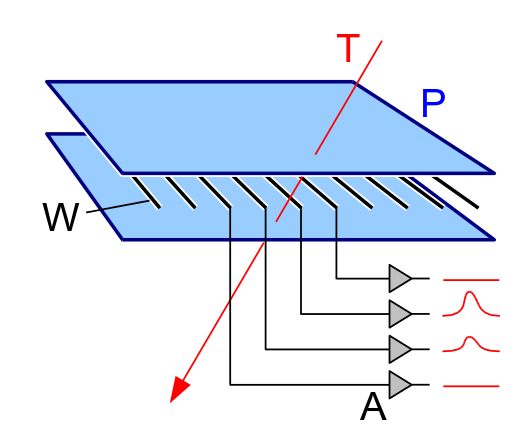
\includegraphics[width=0.5\hsize]{figures/Wire_chamber_schematic.png}}
\legend{A schematic of a multiwire proportinal chamber. The blue plates are the cathodes and the wires are the anodes. When the a particle ionises the gas, the electrons drift towards the wires and, because of the avalanche multiplication, many electron are collected and a measurable signal is obtained at the anodes.}
\source{\cite{wiki:wire}}
\end{figure}

Parallel-plate geometry detectors tend to perform better on this area, because the electric field is uniform, so that all the gas volume is available for amplification, providing excellent timing capabilities \cite{PARKHOMCHUCK1971269}. A successful implementation of the parallel-plate geometry are the resistive plate chambers.

\section{Resistive Plate Chambers}

The RPC was created in 1981 by Santonico and Cardarelli \cite{santonico1981development}. This detector is very similar to a spark chamber, but with a major difference, its electrodes are made of materials with high electrical resistivity, in the order of $10^{10}-10^{12} \; \Omega$cm, made with high pressure laminate (HPL), also known as Bakelite, or glass. The electrodes are coated with a conductive layer to provide good connection to the applied high voltage (HV). 

The two plates form a region where a mixture of gases is flushed, denominated gas gap. The thickness normally goes from 1-2 mm\footnote{Some designs have lower thickness, for instance, check \cite{Deppner:2016yku}} and it is maintained constant by a network of spacers distributed throughout the plane. The signal readout is independent of the HV, it can be performed by copper strips or pads where the avalanche induces signals. A typical design of a RPC chamber is shown in Fig. \ref{fig:RPC_schematic}.

\begin{figure}[!htm]{15cm}
\caption{Resistive Plate Chamber Schematic}%
\label{fig:RPC_schematic}
\fbox{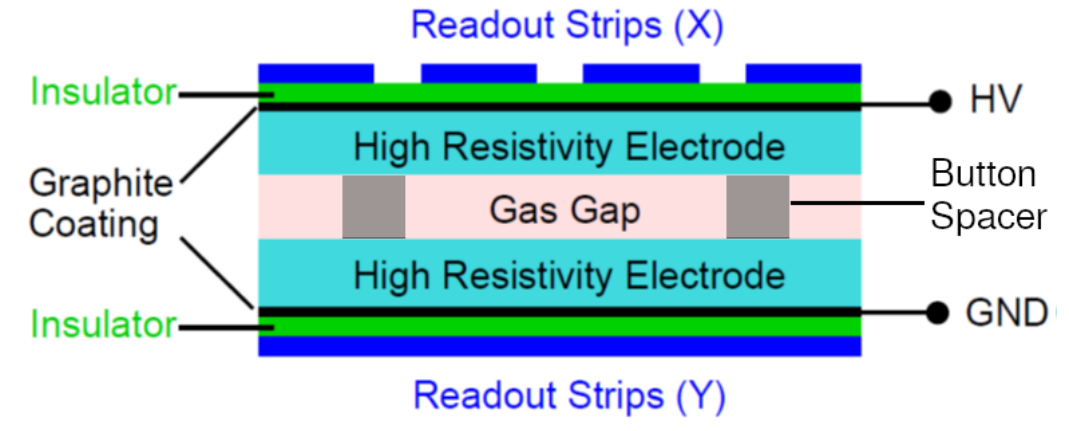
\includegraphics[width=0.5\hsize]{figures/RPC_schematic.png}}
\legend{A Schematic of a typical RPC with one gap and readout by strips in two directions}
\source{\cite{Mondal:2018eov}}
\end{figure}

The gas mixture is very important for efficient operation of the RPC. Normally, a mixture of tetrafluoroethane (C$_2$H$_2$F$_4$, commercially known as R134a or Freon) to enhance ionization of the incident particles, that can compose more than 90\% of the mixture, isobutane (iC$_4$H$_10$) as a quencher gas and (SF$_6$) to improve the electronegativity of the mixture and reduce the secondary ionization. Nowadays, the search of eco-friendly gas mixtures is very important research field for the RPCs. The replacement is very important for the R134a and SF$_6$ as they contribute the most to the high global warming potential (GWP) of the mixture. The commercial replacement to the R134a are the HydroFluoroOlefyns (HFOs), for example the HFO1234ze (C$_2$H$_2$F$_4$) which brings the HV working point (WP) of the RPCs to higher values. Normally, it is added CO$_2$ or Helium to the HFO to bring the WP to a lower level. For the SF$_6$ some gases are being researched, for example, 3M Novec 5110, 3M Novec 4710, AMOLEA HFO-1224yd, etc. More details on the eco gas research can be found in \cite{Guida:2022pyg}. Some alternatives to reduce the flushing of fresh gas into the system, such as gas re-circulation systems, are also being developed \cite{Corbetta:2020esl}.

The detector operates on a very high electrical field strength, in the order of 4-5 kV/mm. The authors of \cite{Santonico:1988qi} pointed out that, when a particle passes by the gas volume, the primary electron-ion pairs gives rise to a small discharge that is quenched without affecting the whole gas volume by the following mechanisms:
\begin{itemize}
    \item Reduction of the electric field in the electrode at the region close to the discharge development, due to the high resistivity electrodes;
    \item Absorption of the UV photons created in the discharge by the isobutane, preventing secondary discharges;
    \item Capture of the electrons in the outer region of the discharge because of the high electronegativity of the Freon.
\end{itemize}

Because of these mechanisms, the discharges in the RPC are not harmful, not destroying the chamber or the front-end electronics. Furthermore, the size of the region affected by the discharge is small, leaving the rest of the chamber active, so that it can sustain higher rates. Coupling these characteristics to the excellent time resolution (some designs in the order of 50 ps) good spatial resolution (up to 50 $\mu$m state of art designs \cite{Francke:2002wq}) and the relatively easy construction and cheap construction, the RPCs are very well suitable for high energy physics experiments, even for tracking. Normally, they are employed in muon systems, where it can cover an area of thousands of square meters as in the case of the CMS Experiment.

\section{CMS RPC Project}

The CMS RPC system consists in 1056 double-gap chambers operating in avalanche mode. Each gap is constructed with two HPL sheets of bulk resistivity 1-6 $\times 10^{10} \; \Omega$ cm. The HPL sheets are spaced 2 mm apart by a grid of plastic spacers. The internal surfaces of the gaps are coated with a 35 to 45 $\mu$m linseed oil. This treatment improves greatly the performance of the chambers, because it smooths the internal surfaces and quench UV photons \cite{Abbrescia:687074, Lu:2009zzd}. The outside surfaces are coated with a conductive graphite paint, forming the electrodes, and isolated by a PET film. One gap is placed on top of the other with a readout of copper strips placed in between. The layout of a double-gap RPC is shown in Figure \ref{fig:RPClayout}. Everything is placed inside a aluminum case.

\begin{figure}[!htm]{15cm}
\caption{Double-gap CMS RPC layout}%
\label{fig:RPClayout}
\fbox{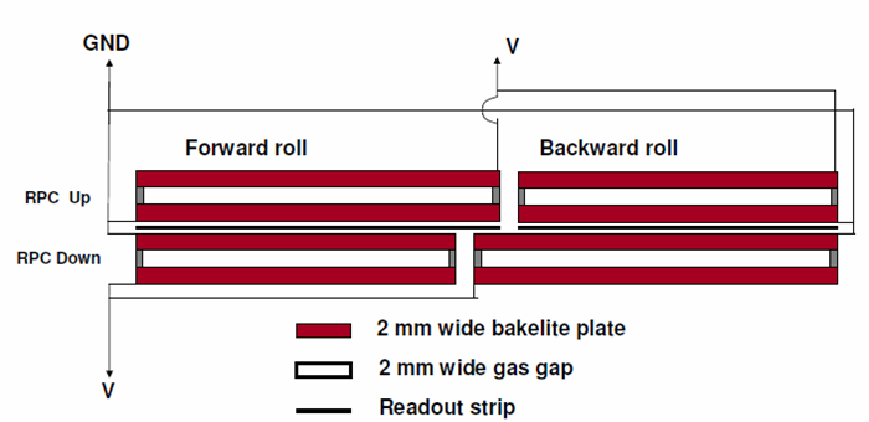
\includegraphics[width=0.5\hsize]{figures/RPC_layout.png}}
\legend{A schematic of a CMS RPC placed in the barrel region. }
\source{\cite{Costantini:1477020}}
\end{figure}

The gas mixture employed, named CMS RPC standard gas mixture, is composed of 95.2 \% of R134a, 4.5 \% of isobutane and 0.3 \% of SF$_6$ kept at 21 $^\circ$C with relative humidity of 40-50 \% to keep the bakelite resistivity stable. 

The RPC system is able to withstand high rate capability of the order of 300 Hz/cm$^2$ a have efficiency greater than 95 \%, cluster size\footnote{number of adjacent strips fired in a single muon hit} less than 2 for a better spatial resolution between 0.8-1.3 cm, the time resolution is 1.5 ns making them interesting for triggering and BX assignment. There are RPCs both in the barrel and the endcap regions of CMS covering an area of 3500 m$^2$. 

\section{CMS RPC Barrel}

In barrel, there are 480 chambers distributed in 5 wheels (Wheel $\pm$ 2, $\pm$ 1 and 0) along the beam pipe. Each wheel consists in 4 stations (RB1-RB4) along the radius. The two inner stations consists of two RPC chambers with a DT in the middle and the two outer stations have only one RPC and one DT. Also, the wheel is divided in 12 sectors (S01-S12) along the direction of the azimuthal angle $\phi$. Due to mechanical reasons, RB3 and RB4 are further divided into two chambers (named + and –) along $\phi$ in all sectors but S04, S09 and S11 in RB4. Since RB4/S09 and RB4/S11 are in the feet of the barrel wheel, they have a single RPC. RB4/S04 have four chambers (named --, -, + and ++). The RPC barrel is given in Figure \ref{fig:RPC_barrel_layout}.

\begin{figure}[!htm]{15cm}
\caption{CMS RPC barrel layout}%
\label{fig:RPC_barrel_layout}
\fbox{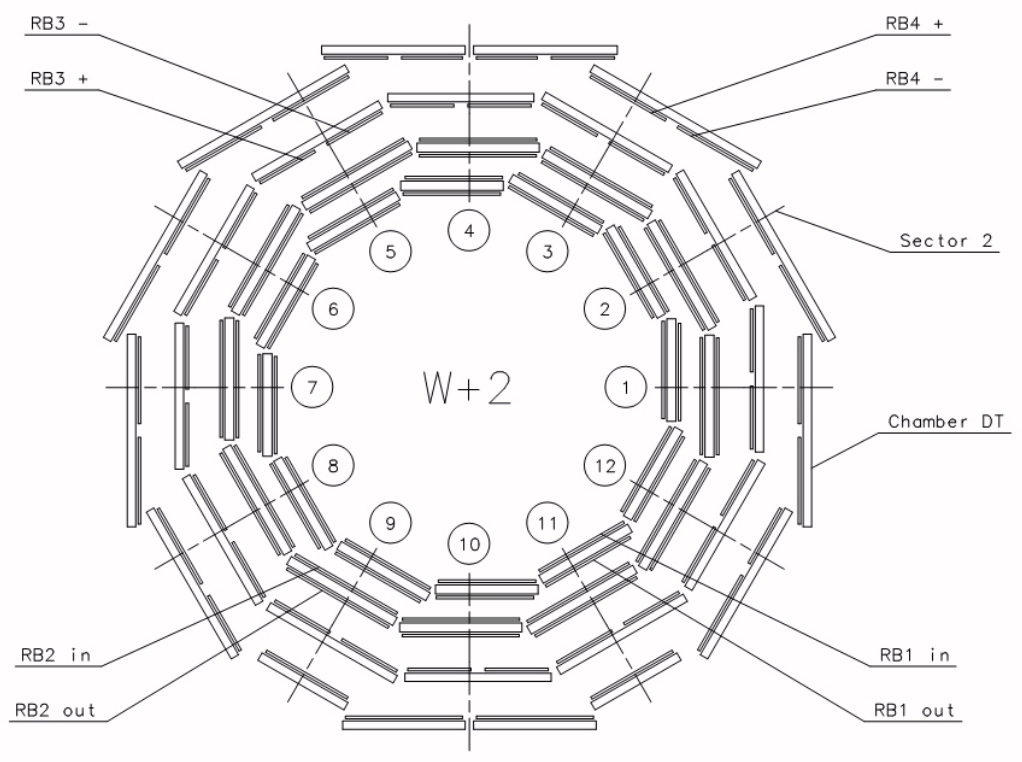
\includegraphics[width=.7\hsize]{figures/RPC_barrel_layout.png}}
\legend{Layout of RPCs placed in the CMS barrel region. They are distributed along 4 stations and 12 sectors for each wheel.}
\source{\cite{CMS:2008xjf}}
\end{figure}

Each RPC chamber is divided into partitions with respect to the pseudorapidity called rolls. Most of the chambers are divided into 2 partitions. Chambers from RB2in in wheels -1, 0 and 1 and RBout in wheels -2 and +2 have 3 rolls. Schematics of this kind of chambers are displayed in Fig. \ref{fig:barrel_chamber_types}.

\begin{figure}[!htm]{15cm}
  \caption{Barrel CMS RPCs division in rolls.} 
  \label{fig:barrel_chamber_types}
  \subfloat[][]{\label{subfig:2rolls}%
    \fbox{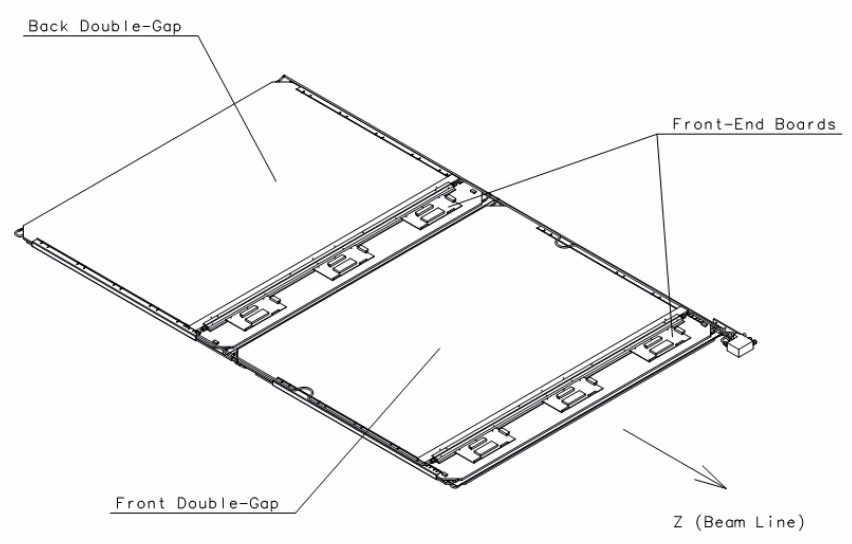
\includegraphics[width=0.45\textwidth]{figures/2rolls_chamber.png}}}\hfill
  \subfloat[][]{\label{subfig:3rolls}%
    \fbox{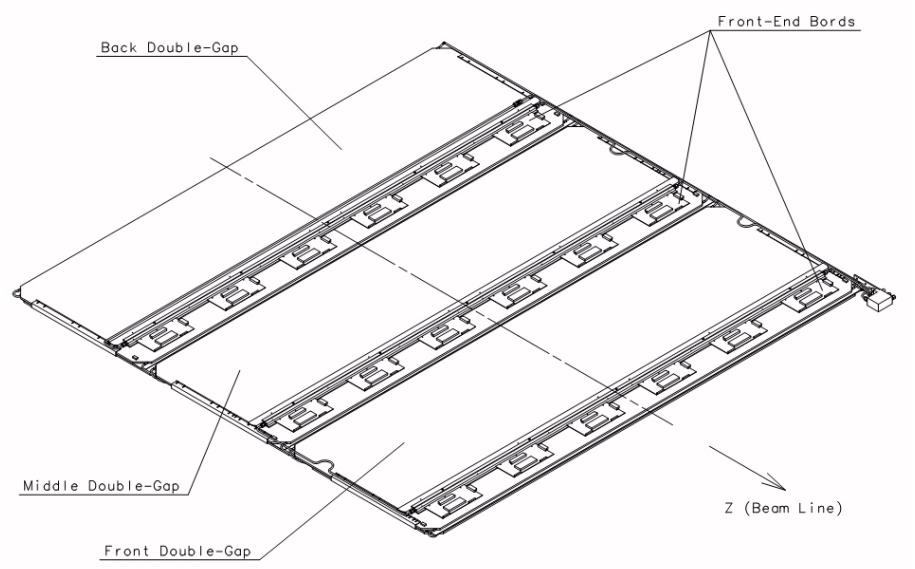
\includegraphics[width=0.46\textwidth]{figures/3rolls_chamber.png}}}\\
  \legend{Layout of chambers in CMS barrel divided into two rolls (a) and three rolls (b).}
  \source{\cite{CMS:2008xjf}}
\end{figure}

\section{CMS RPC Endcap}

In Endcap, there are 576 chambers divided into the 8 disks (RE$\pm$1, RE$\pm$2, RE$\pm$3, RE$\pm$4). Each disk have 72 chambers of trapezoidal shape divided in 2 concentric rings and 36 sectors. Each chamber is divided into 3 rolls, named A, B and C. The higher segmentation with respect to the barrel is driven by the higher particle multiplicity in the frontal regions. A layout of the Endcap geometry is shown in Fig. \ref{fig:RPC_endcap_layout}.

\begin{figure}[!htm]{15cm}
\caption{CMS RPC endcap layout}%
\label{fig:RPC_endcap_layout}
\fbox{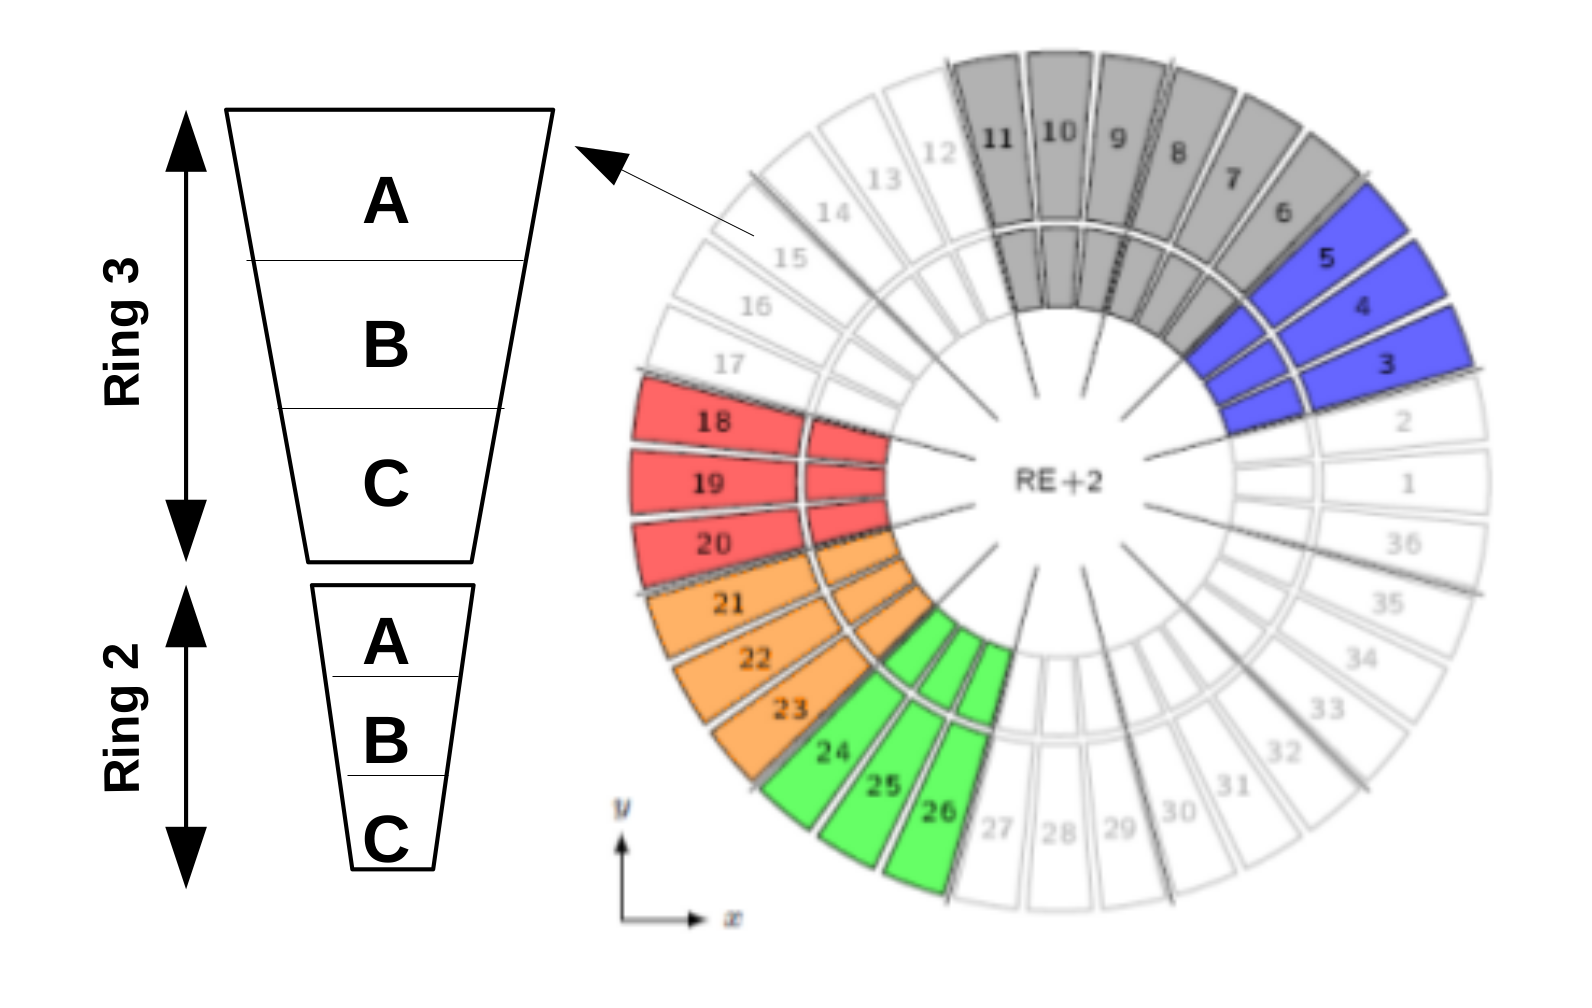
\includegraphics[width=.7\hsize]{figures/RPC_Endcap_layout.png}}
\legend{Layout of a RPCs placed in the CMS endcap region. They are distributed in 2 rings and 36 sectors for each disk.}
\source{\cite{CMSPublic:DPGRPC2016}}
\end{figure}

\section{RPC Upgrade for Phase-2}

The new requirements of the HL-LHC upgrade in terms of pile-up,  background and detector ageing will pose a big challenge for the correct muon identification and transverse momentum determination. The full muon system is preparing upgrades for the HL-LHC. In particular the RPC system is has two important foreseen developments.

The first upgrade is the replacement of the off-detector electronics (called link system). The current link system role is to process, synchronize and zero-suppress the signals coming from the RPC Front-End Boards (FEB) providing the RPC hits in a BX. The new link system will be able to deliver time of the hits, bringing the full timing potential of this detector. Also it will employ techniques and materials to suppress problems and deterioration caused by the high radiation environment.

And the second upgrade is the extension of the RPC coverage from |$\eta$| = 1.9 to 2.4 with the new improved RPC (iRPC) detectors. An extensive R\&D program is taking place to fulfil the demanding conditions of the HL-LHC. Two new RPC layers are going to be installed in the innermost rings of the disks RE$\pm$4 and RE$\pm$3. The new chambers will have a complete new design, with double-gap chambers with 1.4 mm thickness, to improve the time resolution. Also, the readout in two sides of the strip plane, allowing determination of the position in the 2D plane and a completely new front-end electronics. 

Regarding the current system, longevity tests are taking place at CERN GIF++ facility \cite{guida2015gif++}. The chambers are irradiated with a 12.6 TBq source in order to simulate the background conditions of the HL-LHC. The chambers showed stable performance with rates up to 600 Hz/cm$^2$ up to 93\% of the expected integrated charge \cite{Aly_2022}.

A complete review of the muon system upgrade can be found in \cite{CERN-LHCC-2017-012}.

\section{Author's contribution on the CMS RPC Project}

During the course of the PhD, there were many opportunities to contribute to the CMS RPC project. This section highlights the author most important contributions.

\subsection{Standard maintenance during Long Shutdown 2}

From December 2018 to March 2022, the LHC machine ceased operation for maintenance and upgrades in the accelerator complex in a period called Long Shutdown 2 (LS2). This time was an important moment for CMS maintenance and upgrades in preparation for the next data taking period (Run-3). In particular, the CMS RPC system underwent a intensive maintenance program to recover as much as possible the defects of the system system. In preparation for the future installation of the iRPCs chambers cooling and cable services for the new detectors were installed.

An extensive HV and low voltage (LV) maintenance campaign was performed. The goal of HV maintenance was to identify the problematic parts of the HV power system and to fix it in the best possible way, recuperating the performance of the chambers. A RPC chamber can have problems in one of the gaps or both, when the problem is in one of the gaps the efficiency pf such chamber can decrease as much as 15 \%, but it is recoverable with the increase of the applied HV, although it is not optimal as the current increases and the chamber's longevity is affected. 

The problems in HV were normally in one of the HV connectors, either because of bad connection, which was solved by a proper connection, or by defective connector, as shown in Fig. \ref{fig:HV_crack}. If this was the case, a the replacement of the connector or the use of spare channels was enough to bring back the gap to a good performance. In some cases the gaps itself were problematic, for example, because of problems with gas leakage. A total of 65 HV channels were repaired during LS2. 

\begin{figure}[!htm]{15cm}
\caption{Defective HV connector}%
\label{fig:HV_crack}
\fbox{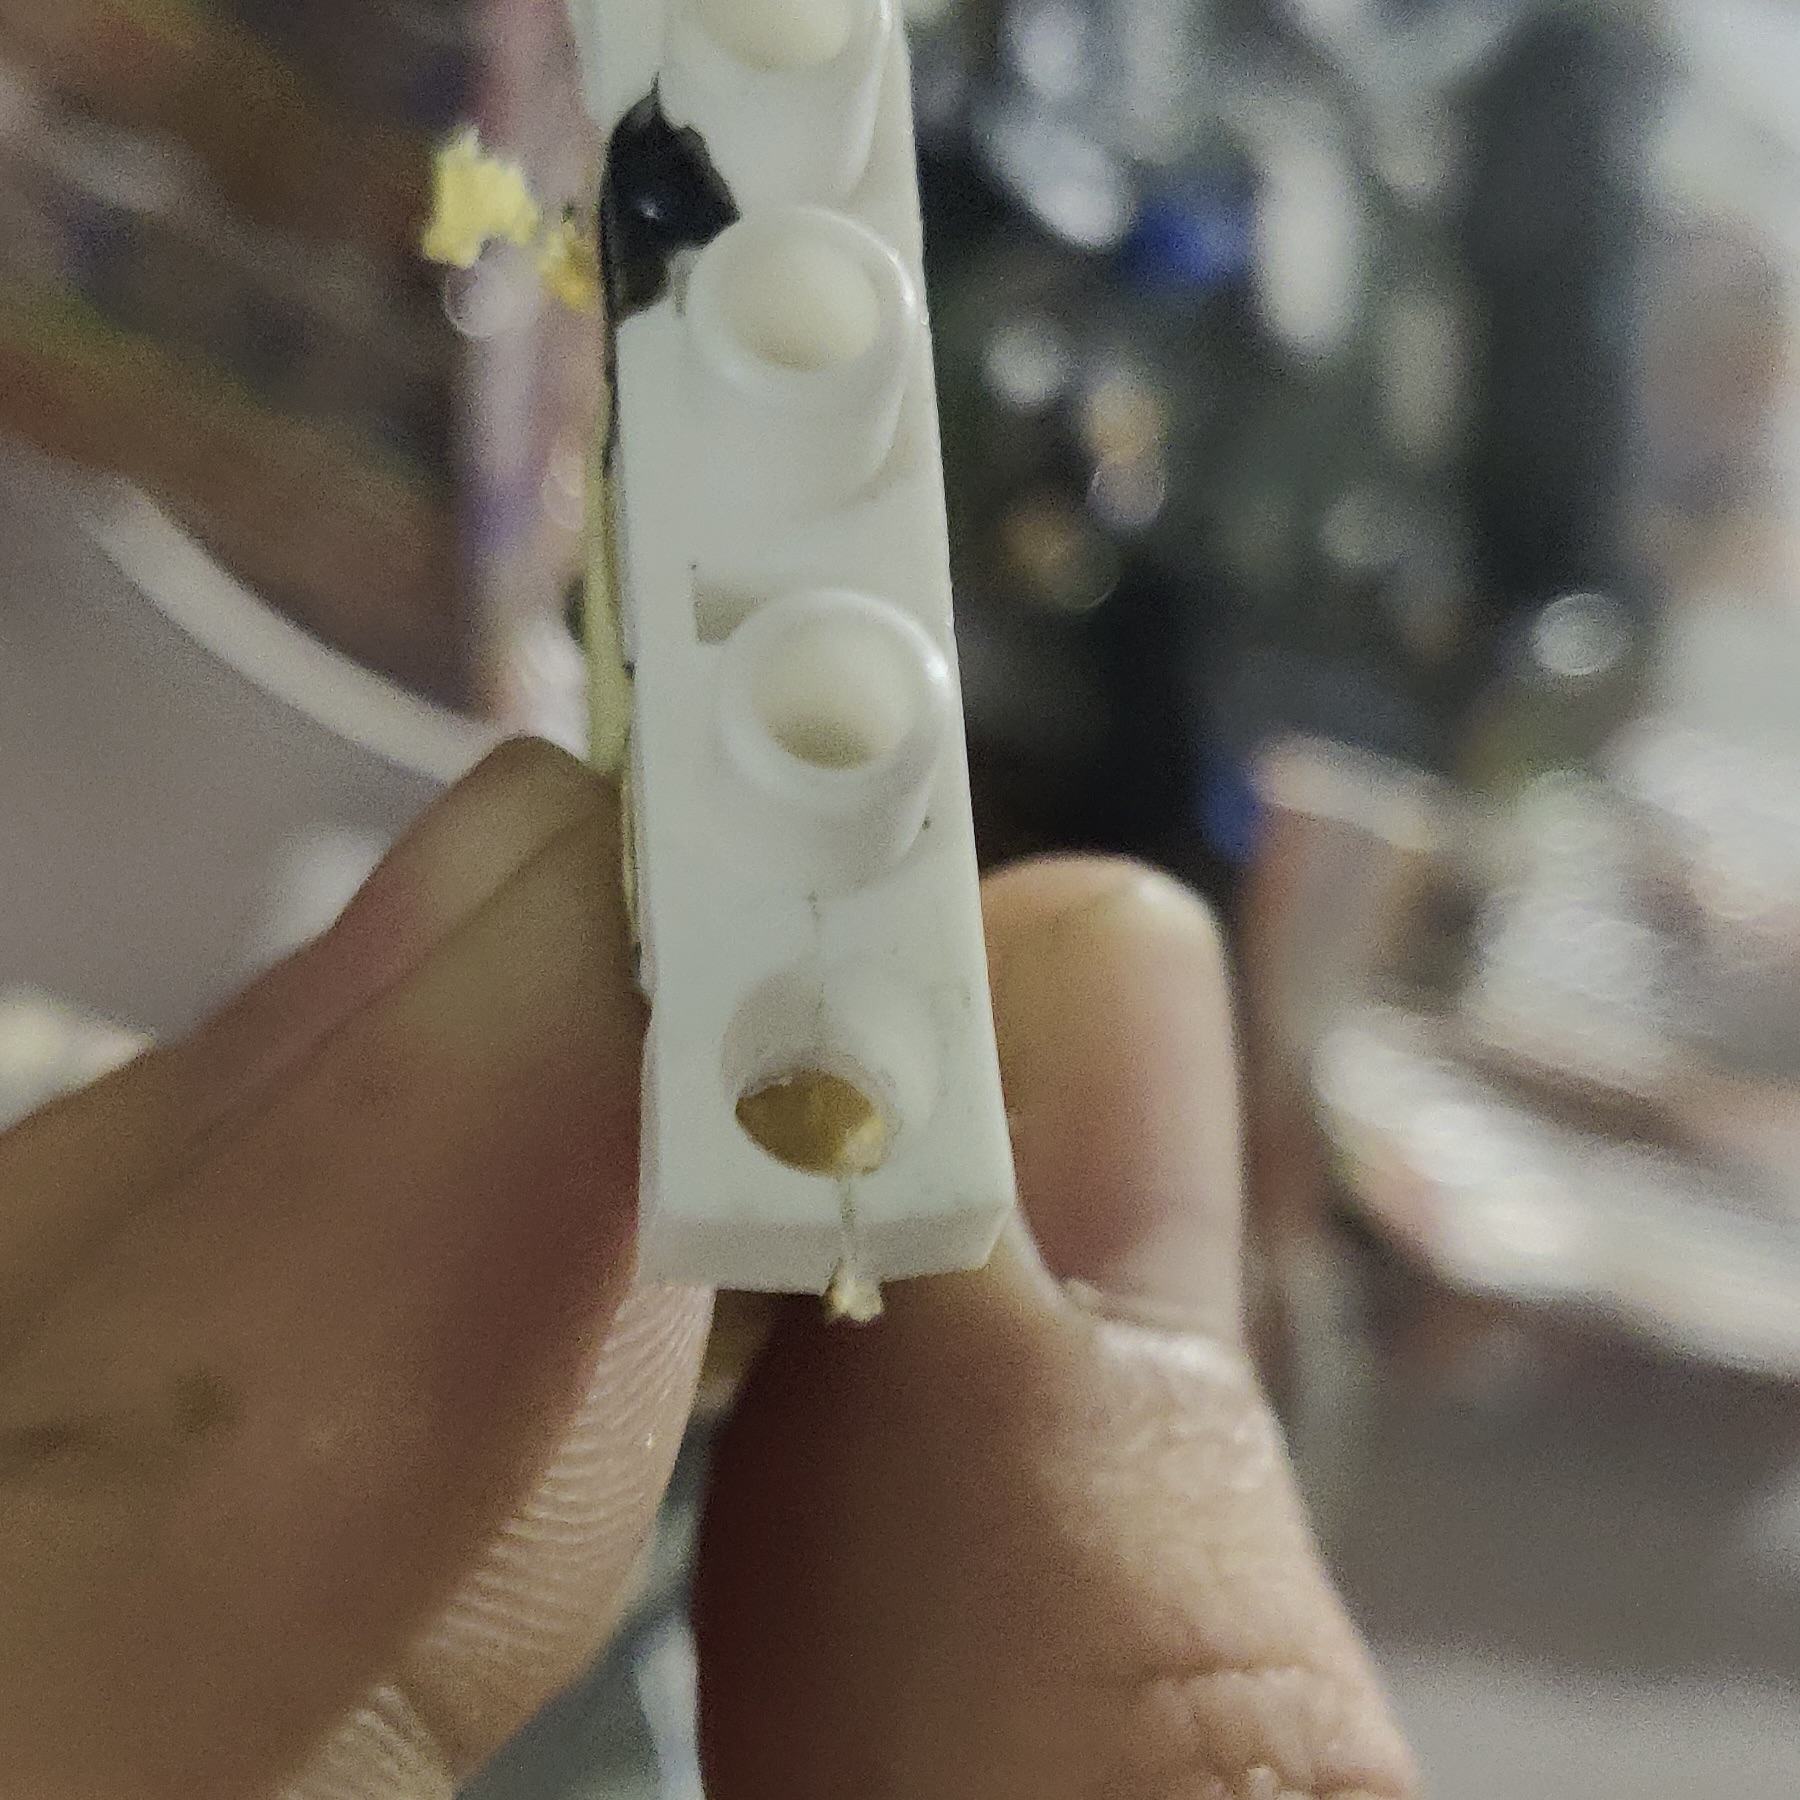
\includegraphics[width=.7\hsize]{figures/HV_crack.jpg}}
\legend{Example of defective HV connector. It is possible to see a crack in the connector on the bottom of the image. This problem compromises the proper isolation of the HV connector, leading to sparks.}
\end{figure}

The LV maintenance aim was to ensure a proper operation and configuration of the detector electronics and ensure a good functionality of the LV power boards and communication buses. A total of 12 LV problems were fixed.

Another important activity was the extraction of the chambers from the two RE4 stations to allow the CSC ME4/1 chambers extraction for electronics  refurbishment. The chambers were brought to the surface, and accommodated to a new laboratory with controlled environmental conditions and the infrastructure needed to test them (HV, LV and gas). All needed reparation and re-validation was done in this laboratory, before all the chambers were installed back.

The most priority activity, was gas system consolidation. The aim was to minimize the environmental impact of the RPC system. The actions taken were:
\begin{itemize}
    \item Gas Leak identification and repair. Often, the problems with the gas leaks were because of broken gas pipes and inlets inside the chambers. A endoscope was employed to find the problematic points and reparation was done when accessible. Figure \ref{fig:gas_problems} shows examples of problems found with the endoscope. Out of the identified 122 leaky chambers in barrel 49 where repaired, 14 are non-recoverable.
    \item Recuperation of the Exhaust, which was not working during Run-2 for the installation of the first C2H2F4 recuperation system with efficiency of 80 \%, which have been developed by CERN EP-DT Gas team \cite{Corbetta:2020esl}.
    \item Installation automatic pressure regulation valves on the redistribution gas racks to minimize pressure variations in the chambers, which can be a possible source of new leaks.
    \item Turn off the remaining leaky chambers which was not possible to repair, to keep the amount of fresh gas added to the system at a minimum.
\end{itemize}
A summary of the activities in LS2 can be found in \cite{Amarilo_2022}.

\begin{figure}[!htm]{15cm}
  \caption{Gas problems inside RPC chambers.} 
  \label{fig:gas_problems}
  \subfloat[][]{\label{subfig:gas_crack}%
    \fbox{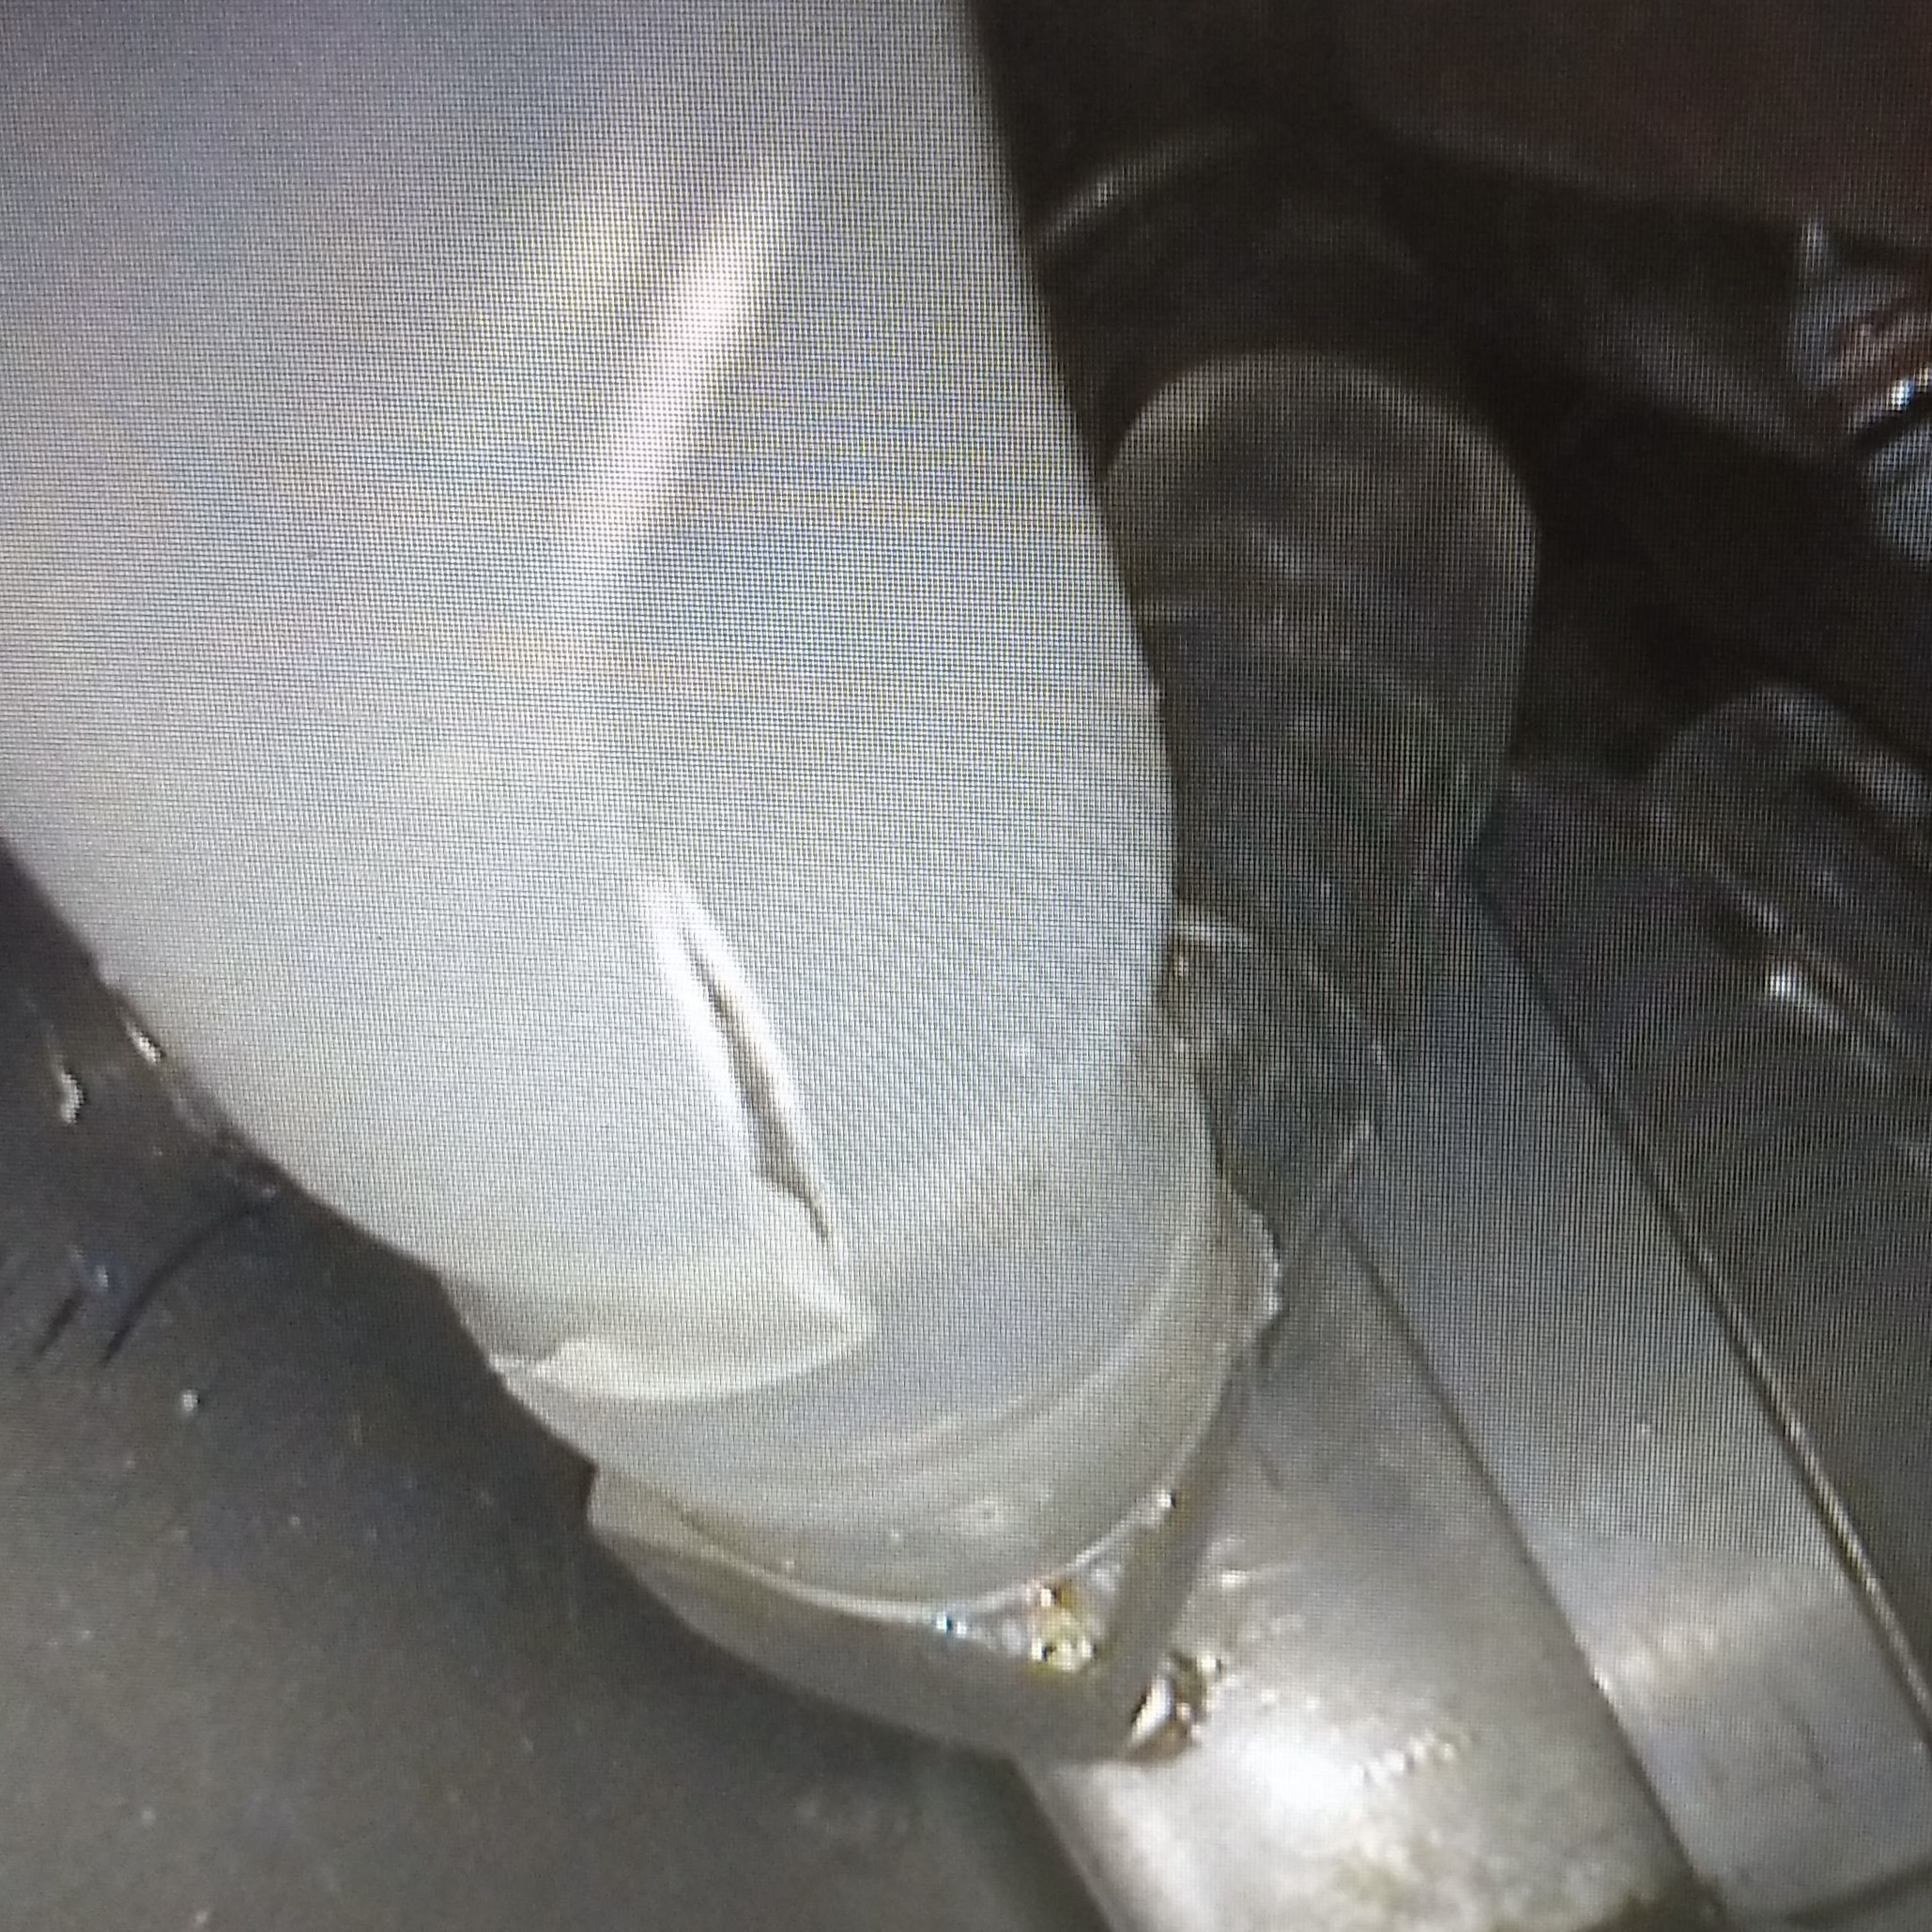
\includegraphics[width=0.45\textwidth]{figures/gas_crack.jpg}}}\hfill
  \subfloat[][]{\label{subfig:gas_break}%
    \fbox{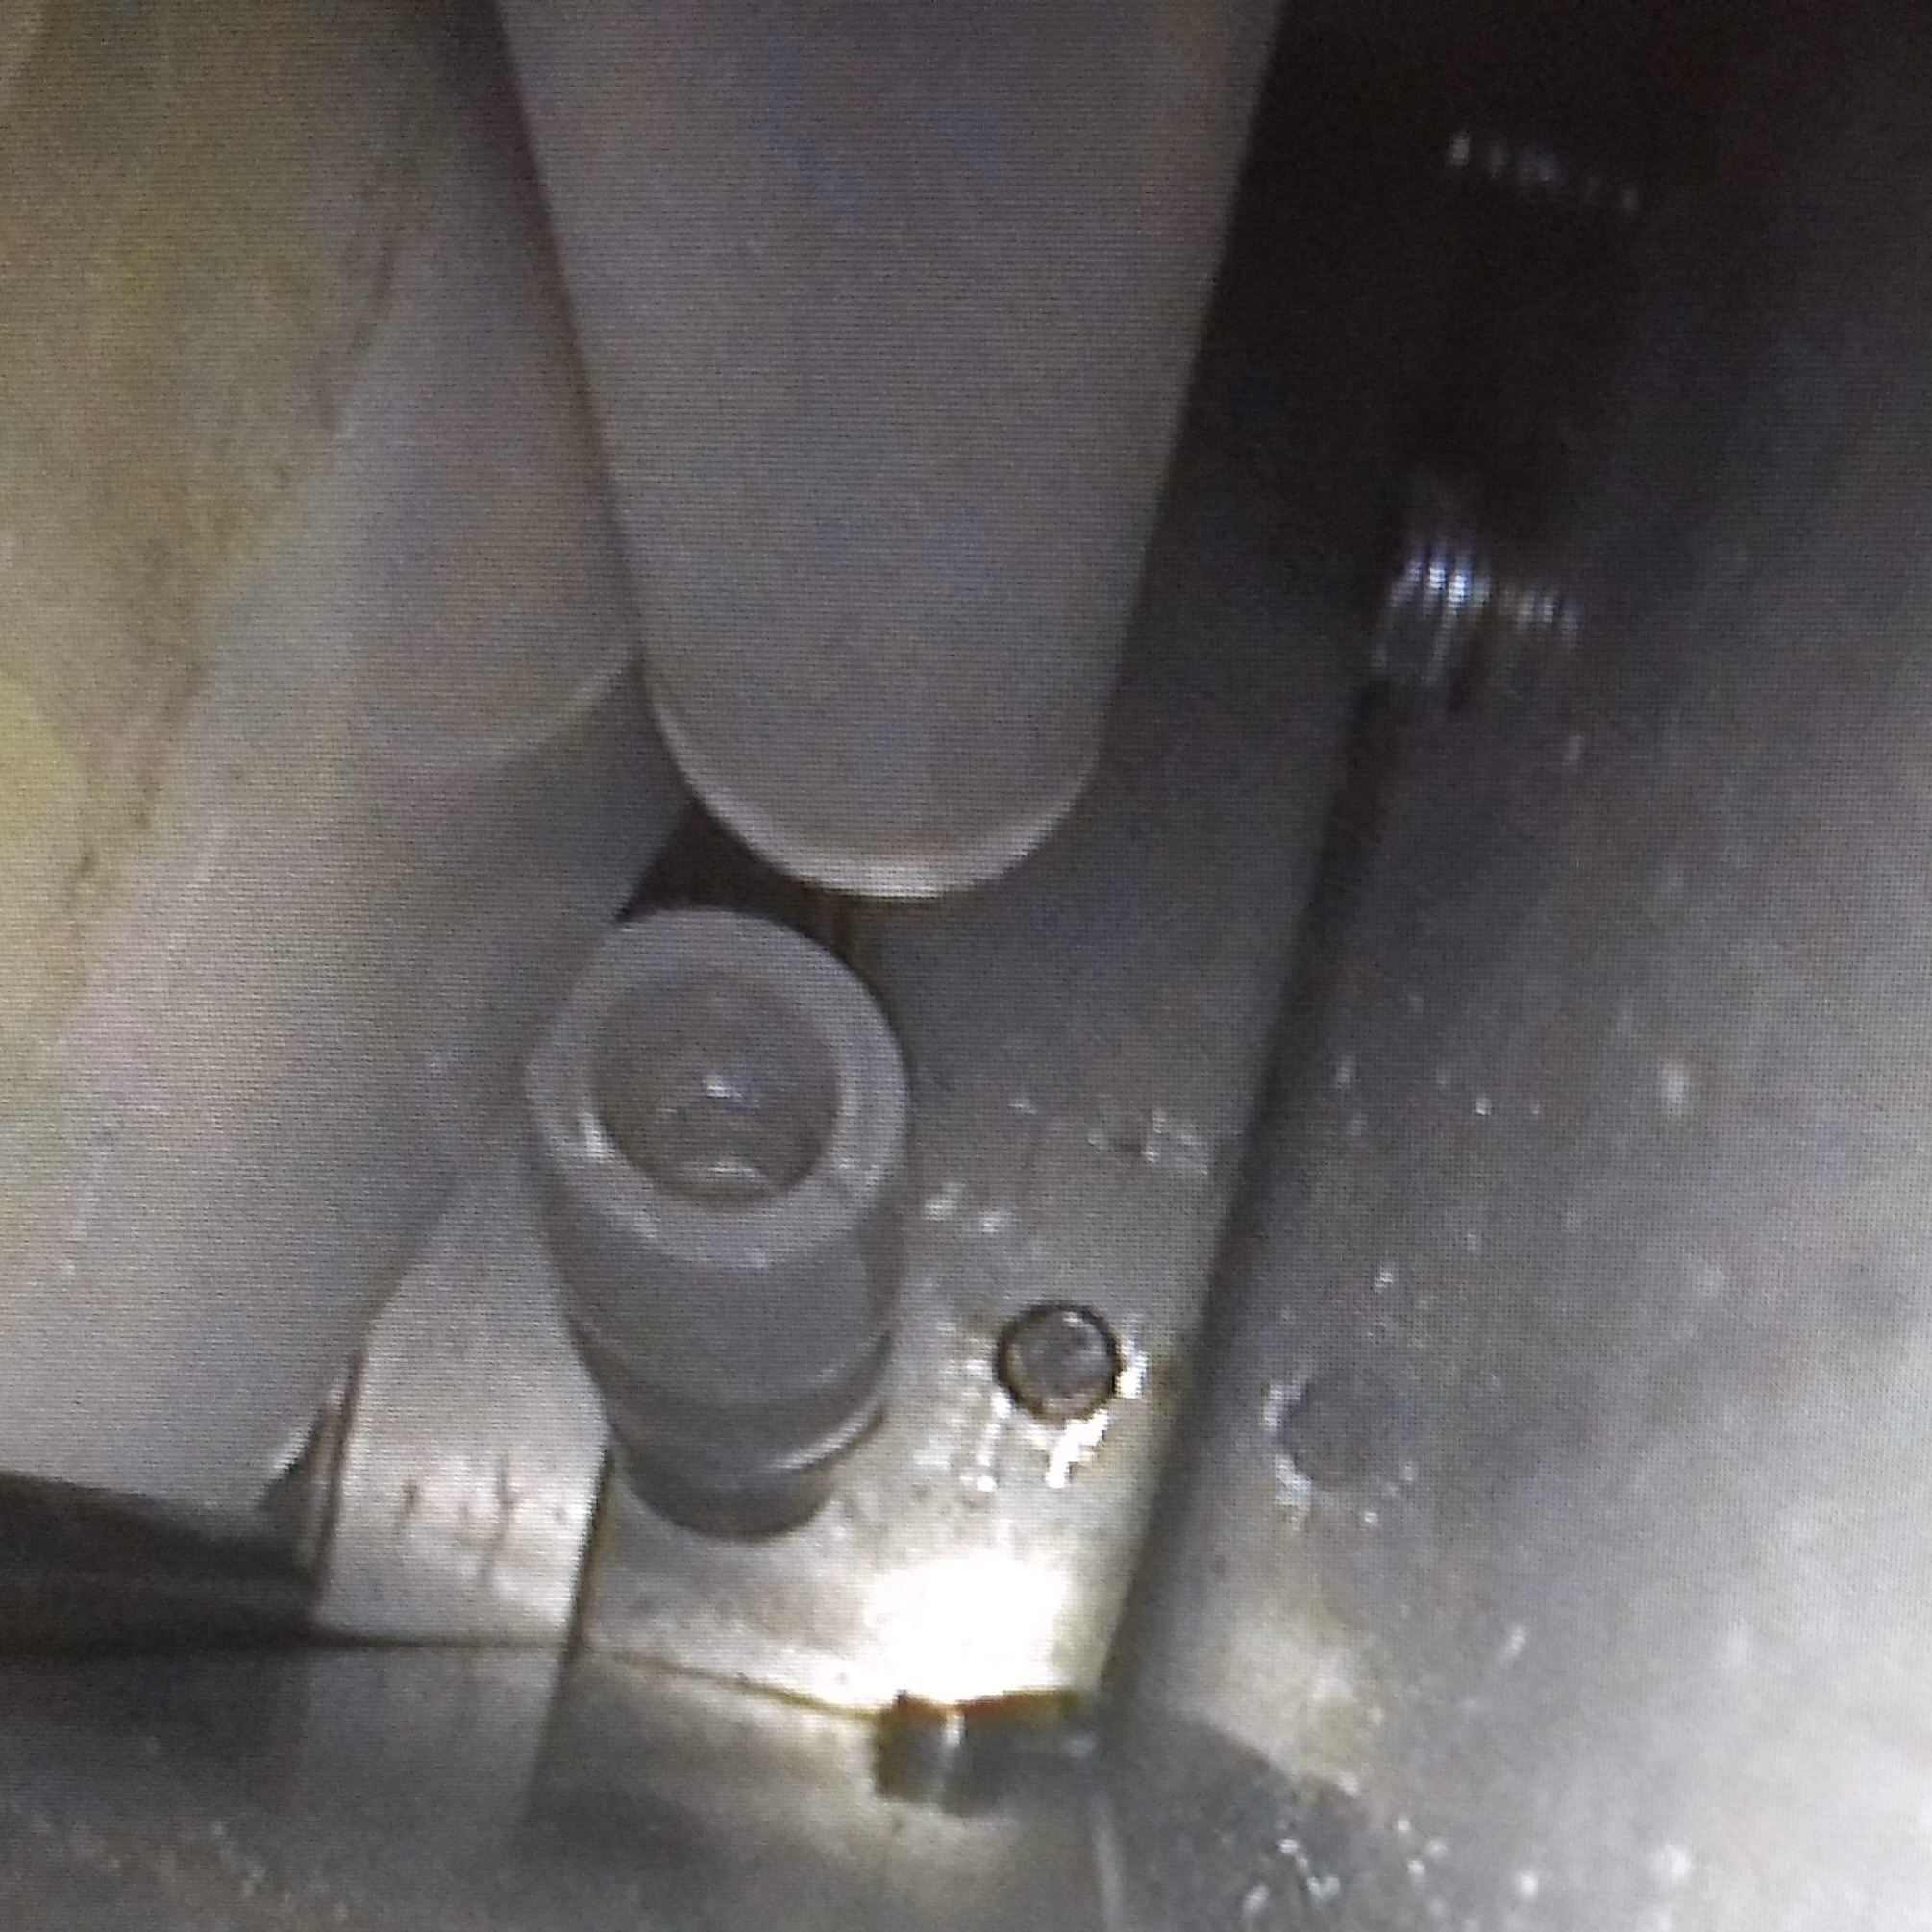
\includegraphics[width=0.45\textwidth]{figures/gas_broken.jpg}}}\\
  \legend{Pictures taken during endoscopic inspection to find gas problems inside RPC chambers. a crack in the pipe is found in (a) and a completely cut pipe in (b)}
\end{figure}

The performance of the repaired chambers can be seen in Figs. \ref{fig:repaired_gas} and \ref{fig:repaired_HV} as a comparison between cosmic-rays data-taking of 2018 and 2021. There was great improvement, 34 rolls were recovered by gas leak repairs and the HV repairs translated into a gain of ~6\% in the efficiency of these chambers. Overall, the results of the repairs were successful bringing higher efficiency to the repaired channels. In Fig. \ref{fig:overallefficiency2018vs2022} a comparison of the distribution of roll efficiency in pp collisions taken in 2018 and 2022 is given for barrel and endcap and the results mentioned are confirmed.

\begin{figure}[!htm]{15cm}
\caption{Performance of repaired gas leak chambers in cosmic data taking}%
\label{fig:repaired_gas}
\fbox{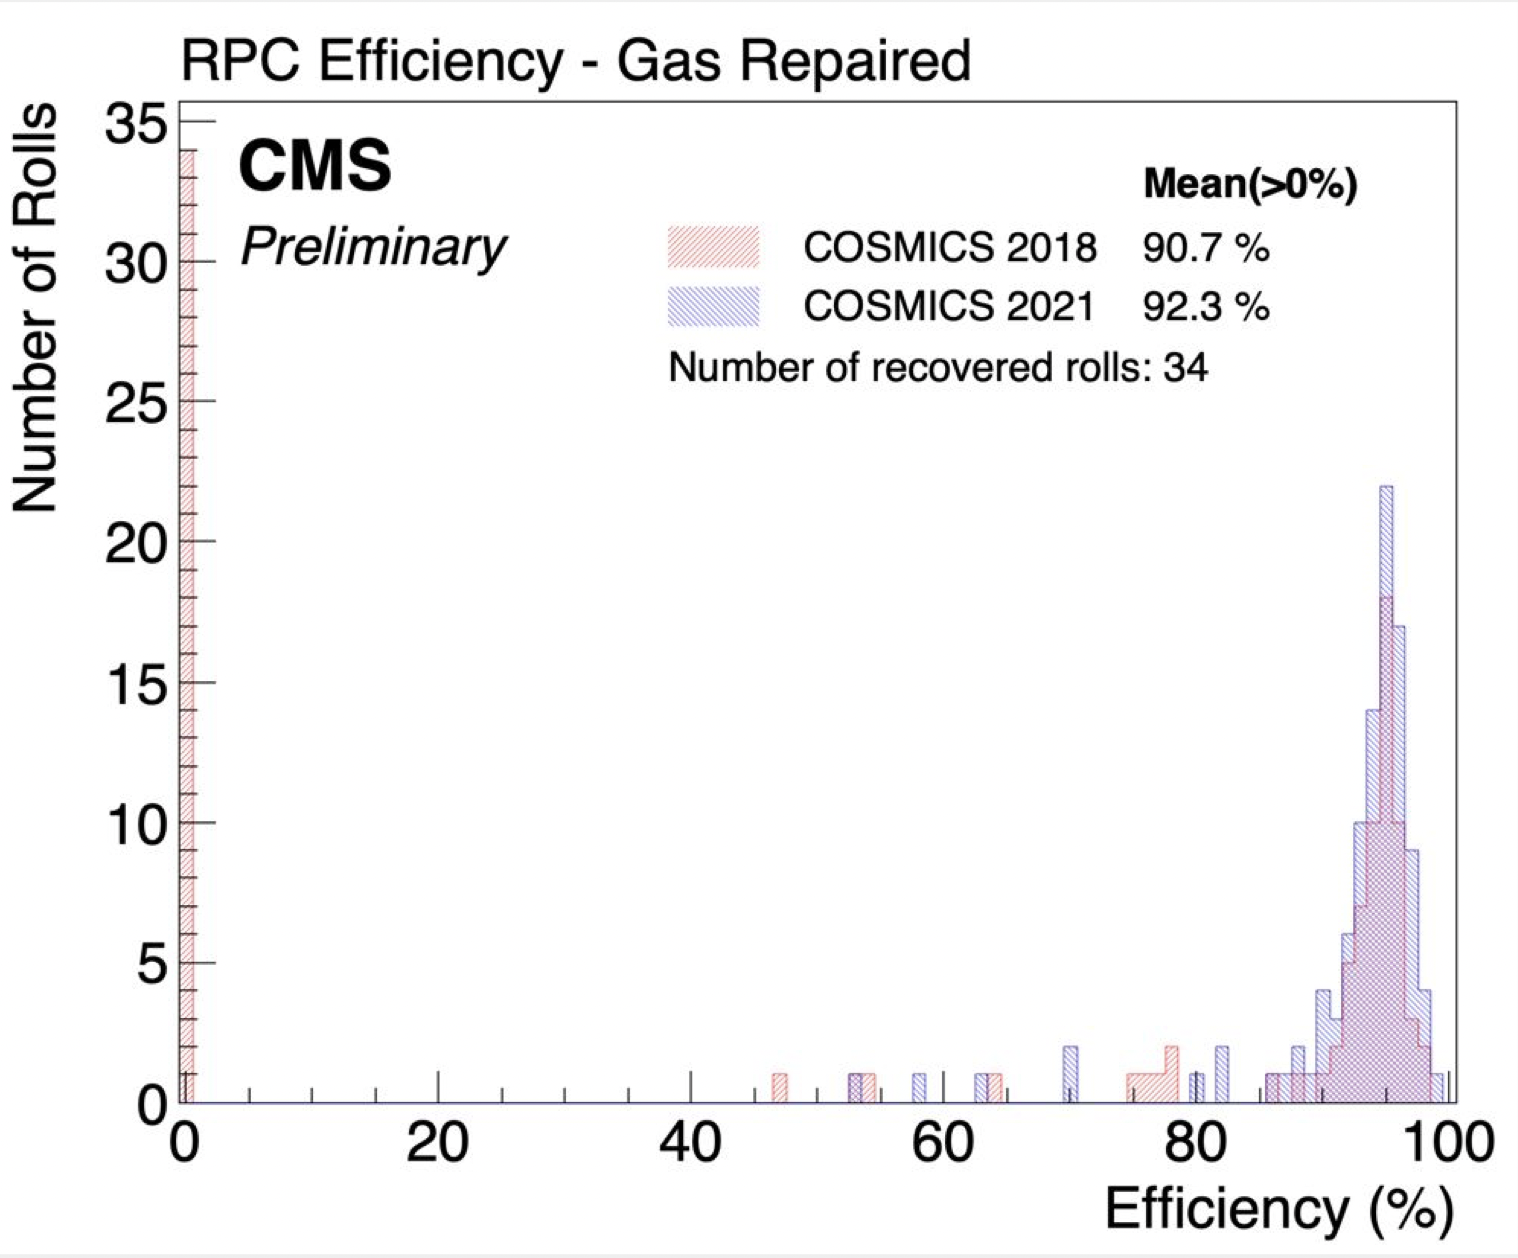
\includegraphics[width=.5\hsize]{figures/Repaired_gas.png}}
\legend{The distribution of efficiency of RPC rolls on gas repaired chambers during the Long Shutdown 2 (LS2). Using cosmics data taking in 2018 (red) and 2021 (blue) for barrel region. The numbers show a significant improvement, with respect to 2018 as 34 OFF rolls from Run-2 are recovered and HV is repaired for several chambers recovering chambers from Single Gap to Double Gap operation mode.}
\source{\cite{CMSPublic:DPGRPC2021}}
\end{figure}

\begin{figure}[!htm]{15cm}
\caption{Performance of repaired gas leak chambers in cosmic data taking}%
\label{fig:repaired_HV}
\fbox{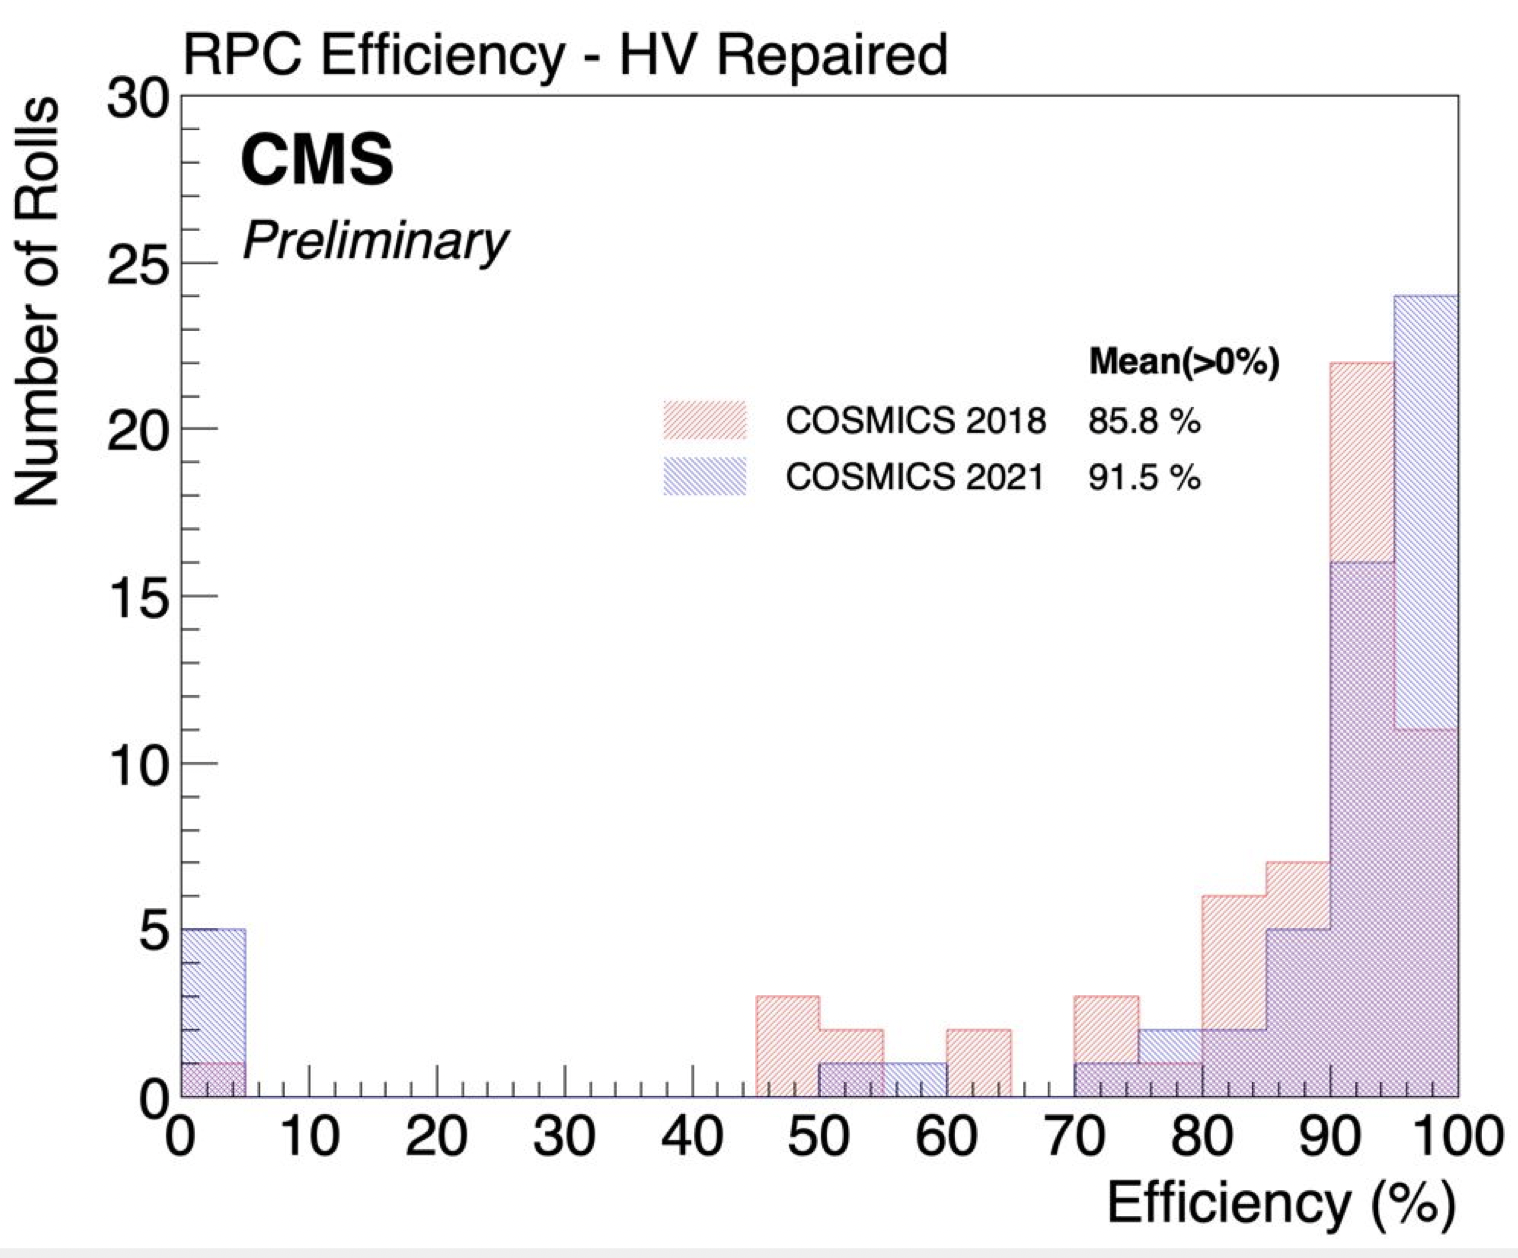
\includegraphics[width=.5\hsize]{figures/Repaired_HV.png}}
\legend{The distribution of efficiency of RPC rolls on HV repaired chambers during the Long Shutdown-2 (LS2) using cosmics data taking in 2018 (red) and 2021 (blue) for barrel region. The RPC efficiencies measured in 2021, after LS2 are comparable and in agreement with the expectations. The overall efficiency is improved by ~6\% due to recovery of chambers from Single Gap to Double Gap operation mode.}
\source{\cite{CMSPublic:DPGRPC2021}}
\end{figure}

\begin{figure}[!htm]{15cm}
  \caption{Overall RPC efficiency in pp collisions.} 
  \label{fig:overallefficiency2018vs2022}
  \subfloat[][]{\label{subfig:overallefficiency2018vs2022barrel}%
    \fbox{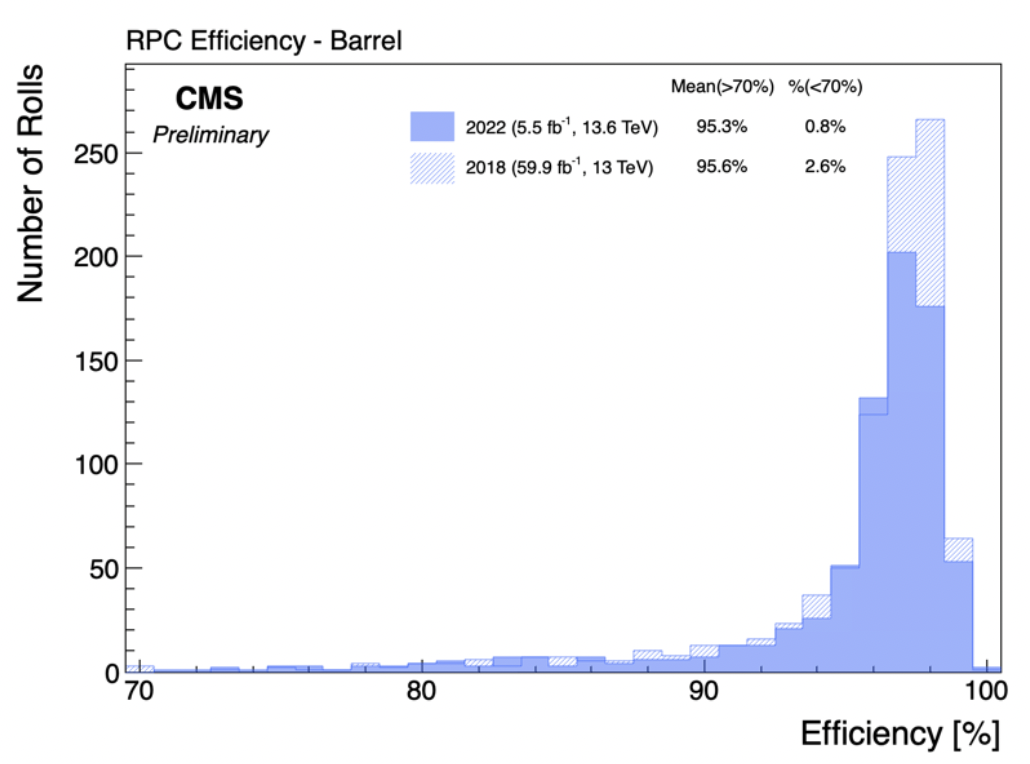
\includegraphics[width=0.45\textwidth]{figures/Efficiency_Barrel.png}}}\hfill
  \subfloat[][]{\label{subfig:overallefficiency2018vs2022endcap}%
    \fbox{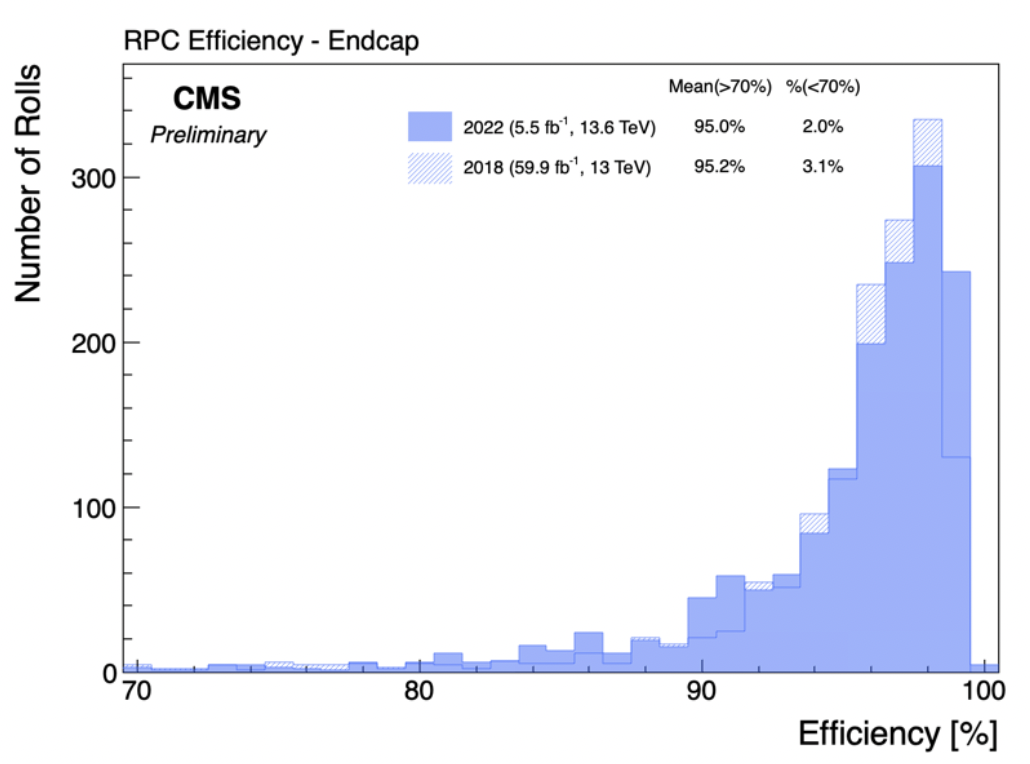
\includegraphics[width=0.45\textwidth]{figures/Efficiency_Endcap.png}}}\\
  \legend{Comparison of the overall RPC efficiency in 2018 and 2022 in pp collisions data taking. The barrel chambers are plotted in (a) and the endcap ones in (b).}
  \source{\cite{CMSPublic:DPGRPC2022}}
\end{figure}

\subsection{RPC Detector Control System}

A big experiment like CMS need a control software for all the required needs for control, monitoring and safe operation of its subsystems. The WinCC\footnote{formerly known as PVSS} SCADA (Supervisory Control And Data Acquisition) software together with the Joint Control Project (JCOP) framework form the basis of the Detector Control System (DCS) for the big experiments at LHC \cite{Arcidiacono:2005fr}. 

Each subsystem at CMS is tasked to develop the DCS for itself to be able to react to the commands passed from the CMS Central DCS. The RPC DCS is divided into several subsystems that are part of the infrastructure needed for the operation of the RPCs chambers as shown in Figure \ref{fig:RPC_DCS_layout}. Each subsystem communicates with DCS, passing information that is archived in a ORACLE database and receiving commands.

\begin{figure}[!htm]{15cm}
\caption{CMS RPC DCS layout}%
\label{fig:RPC_DCS_layout}
\fbox{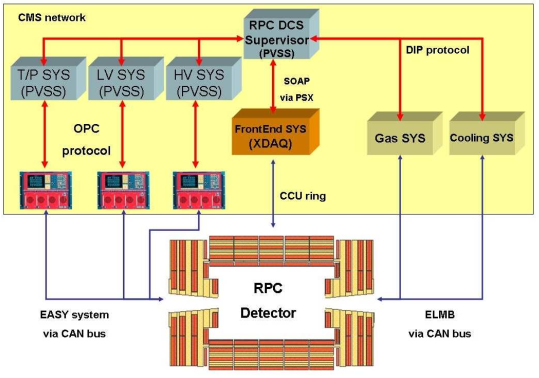
\includegraphics[width=\hsize]{figures/RPC_DCS_subsystems.png}}
\legend{The CMS RPC DCS layout, displaying all its subsystems.}
\source{\cite{Polese:2010zz}}
\end{figure}

The Power system for HV and LV is based on the CAEN EASY project \cite{CAENEASY}. It is designed to operate in hostile areas (high radiation and magnetic field strength) and connected to the DCS through the OPC protocol \cite{OPCFoundation}.  Temperature and relative humidity (RH) sensors are read by ADCs connected to the CAEN EASY system and sent to DCS. The gas infrastructure data is acquired from Programmable Logic Controllers and distributed via DIP \cite{Barillere:2003fi}. In the same way all the information concerning the CMS infrastructure, (e.g. Cooling, Detector Safety System (DSS), LHC and Magnet status), is available through DIP. Finally, FEB information is available through XDAQ, the online CMS framework, using SOAP (Simple Object Access Protocol)  messages to PSX \cite{gutleber2002software}.

All this control subsystems are able to run by itself as components of the RPC system. However, all the information is gathered around a hierarchical hierarchical double-tree control structure, shown in Fig. \ref{fig:RPC_DCS_structure}, implemented through a Finite State Machine (FSM). This automation schema reduces the amount of human intervention in the system, for all the repetitive tasks, and optimize recovery procedures in case of undesired states. The FSM is defined by its states and the commands. The states are:
\begin{itemize}
    \item ON - RPC is ready for data taking.
    \item STANDBY - High voltages are on standby voltage (6500 V for the CMS RPCs and 5000 V for the iRPCs), low voltages are on. It is used as a safe state.
    \item OFF - Both high voltages low voltages are switched-off.
    \item RAMPING - A transitional state, while the High voltage is moving to the desired set point.
    \item ERROR - A manual intervention is required and no data taking is possible.
\end{itemize}
The commands are ON, OFF and STANDBY, which effectuates the transitions to the states with same name.

\begin{figure}[!htm]{15cm}
\caption{CMS RPC hierarchy tree}%
\label{fig:RPC_DCS_structure}
\fbox{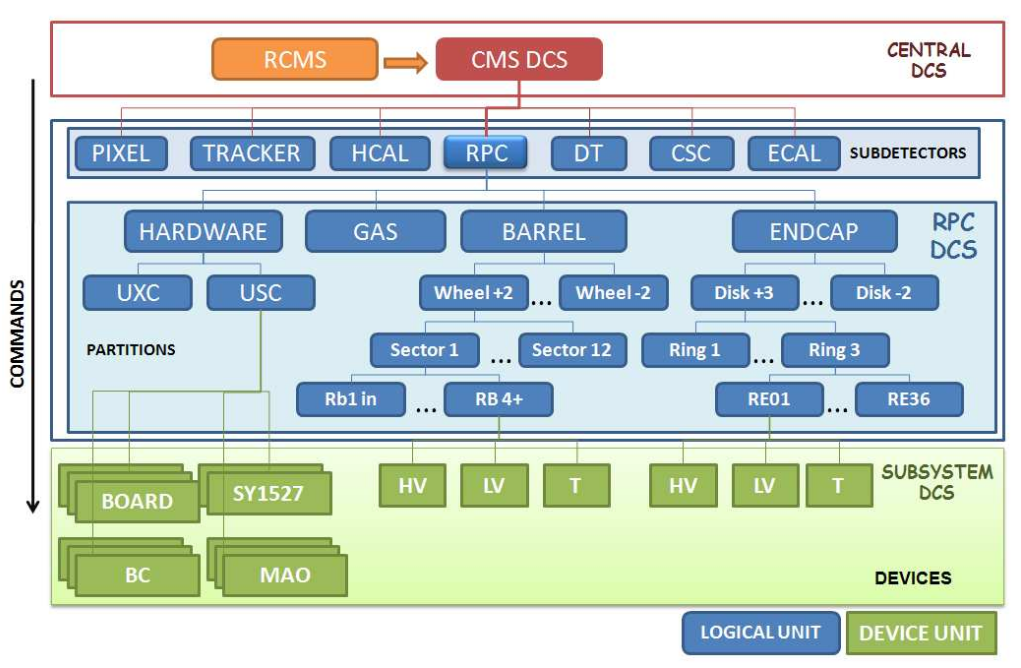
\includegraphics[width=\hsize]{figures/RPC_DCS_Structure.png}}
\legend{Structure of the hierarchy tree of the RPC DCS. Different branches describe the
RPC system from the geographical and hardware points of view. All commands go down the
hierarchy, while information and error messages are reported upwards.}
\source{\cite{Polese:2010zz}}
\end{figure}

The WinCC software can also be used to develop a Graphical User Interface (GUI). It is developed to be a easy way for the user interact to the system, being able to control and monitor the desired parameters of the system, as well as display the important alerts. It is structured in approximately 40 panels to provide easy visualization and navigation through the system structure. The GUI can be accessed remotely, which is very important for a collaboration with people from different countries in the world, like CMS, and provides a authentication system, to prevent use from non-experts. Figure \ref{fig:RPC_DCS_GUI} displays a overview of the RPC DCS GUI.

\begin{figure}[!htm]{15cm}
\caption{CMS RPC DCS GUI overview}%
\label{fig:RPC_DCS_GUI}
\fbox{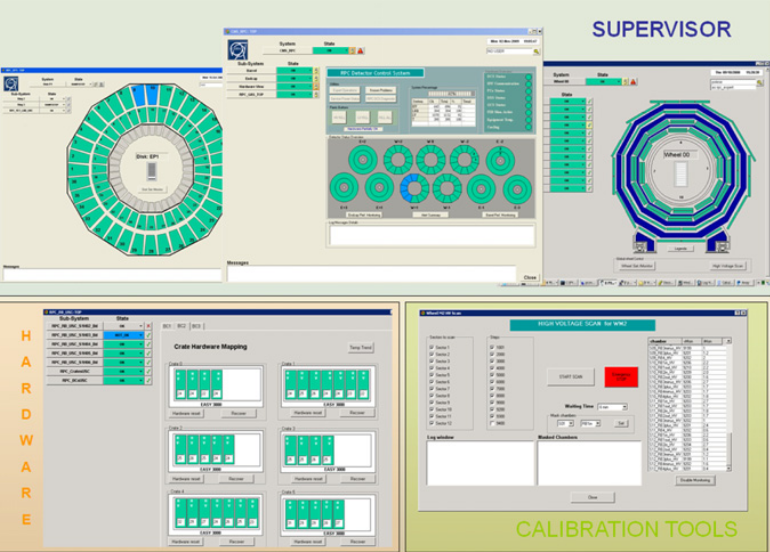
\includegraphics[width=\hsize]{figures/RPC_DCS_GUI.png}}
\legend{Overview of the CMS RPC DCS GUI. The panels are formed with a combination of widgets and texts to better display the system structure.}
\source{\cite{Polese:2012zz}}
\end{figure}

More details on the design of the RPC DCS can be found in \cite{Polese:2010zz, Polese:2012zz}

The work done at the CMS RPC DCS were the update of the system for the upgrade from WinCC version 3.15 to 3.16, which introduced some breaking changes, so the current software needed to be adapted to this new version. The correction of bugs and addition of new functionalities. The most important tasks were the creation of a new panel, shown in Fig. \ref{fig:RPC_DCS_Demo_panel}, for four iRPCs installed as a Demonstrator.

\begin{figure}[!htm]{15cm}
\caption{CMS RPC DCS Demonstrator panel}%
\label{fig:RPC_DCS_Demo_panel}
\fbox{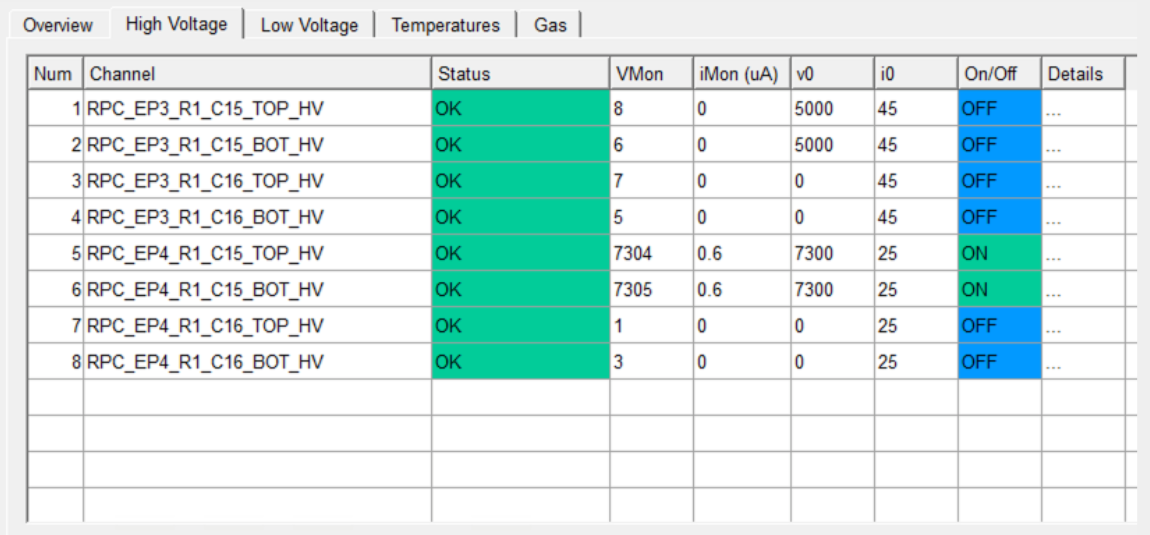
\includegraphics[width=\hsize]{figures/Demo_panel.png}}
\legend{New Panel at CMS RPC DCS for the iRPC demonstrator chambers control and monitoring}
\end{figure}

The most important task was the creation of a new database schema for the gas system. Because of the big changes in the gas system, due to the gas leaks, many channels had to be swapped and some of them switched off. This created the need to change the previous schema, which was chamber-based, to a new one, with abstractions for the gas racks, gas channels and the chambers. Furthermore, the gas flow cells used were found to not be precise enough in the gas flow measurements, that are very important to the determination of whether or not the chambers are leaking. This demanded the creation of three new tables in the database schema and update of the WinCC with the new abstraction. The tables were created also to facilitate the relationship between chambers, the geographical position and infrastructure they use (e.g. HV/LV/gas channels) and current ``health'' situation (any of the gaps are disconnected).

The gas flow for each one of the gas channels were calibrated by a linear function, which parameters were determined for each one of the flow cells by using a very precise mass flow meter. The DCS is also tasked to use these parameters to calculate the corrected flow.

\subsection{RPC-based tracking system at GIF++}

Another task developed for the RPC Project was to help in the test beams at CERN Gamma Irradiation Facility (GIF++), to measure the performance and longevity of the RPC and iRPC chambers in the HL-LHC conditions. 

GIF++ is a very singular facility, where a high energy particle beam (normally muons) and and photons from a gamma source (13 TBq, $^{137}$Cs), with adjustable flux, are combined \cite{guida2015gif++}. Tests for the muon detectors of several experiments (e.g. ATLAS, ALICE, CMS and SHiP) are taking place there.

The chambers must be validated up to the expected background rate: 600 Hz/cm$^2$ for the RPCs in the current CMS Muon system and up to 2 kHz/cm$^2$ for the new iRPCs (including the safety factor of three) \cite{CERN-LHCC-2017-012}. Such high rates can pose a challenge to the measurement, as the fake hits can bias the data-taking. So a tracking system made of RPCs was proposed to remove the background that comes from photons, taking into account the high efficiency of these chambers to muon and the fact that the photon can only be detected by the RPC after being converted to electrons, and the detection efficiency is low (< 1\%) \cite{Weizheng:2014ifa}.

The data acquisition is performed using a CAEN Time-to-Digital Converter (TDC) module of type V1190A where the front-end electronics of the chambers are connected. A V1718 VME controller module is responsible for the communication between the TDC and the computer where the data are stored. To host the VME controller and the TDC a 6U VME 6021 crate is used.

To determine the data taking with respect to the HV, several runs are taken for different HV points. The hits are recorded by the TDC with respect to a trigger based by a coincidence of scintillation detectors, as shown in Figure \ref{fig:RPC_hits_TDC}, all the hits are recorded in a time window of 5 $\mu$s. The triggered muons show a narrow peak in Fig. \ref{subfig:RPC_hits_TDC_muonspill}, so a time window is defined for the hits that are going to be taken into account for the efficiency calculation, in order to suppress the the majority of background from gammas. The time window is defined by doing a Gaussian fit to the time profile in the region of the peak and a window of 6 times sigma, centred in the mean of the fitted Gaussian is taken as the muon window, as given by Fig. \ref{subfig:RPC_hits_TDC_zoomed}.

\begin{figure}[!htm]{15cm}
  \caption{RPC hits recorded by a TDC at GIF++.} 
  \label{fig:RPC_hits_TDC}
  \subfloat[][]{\label{subfig:RPC_hits_TDC_muonspill}%
    \fbox{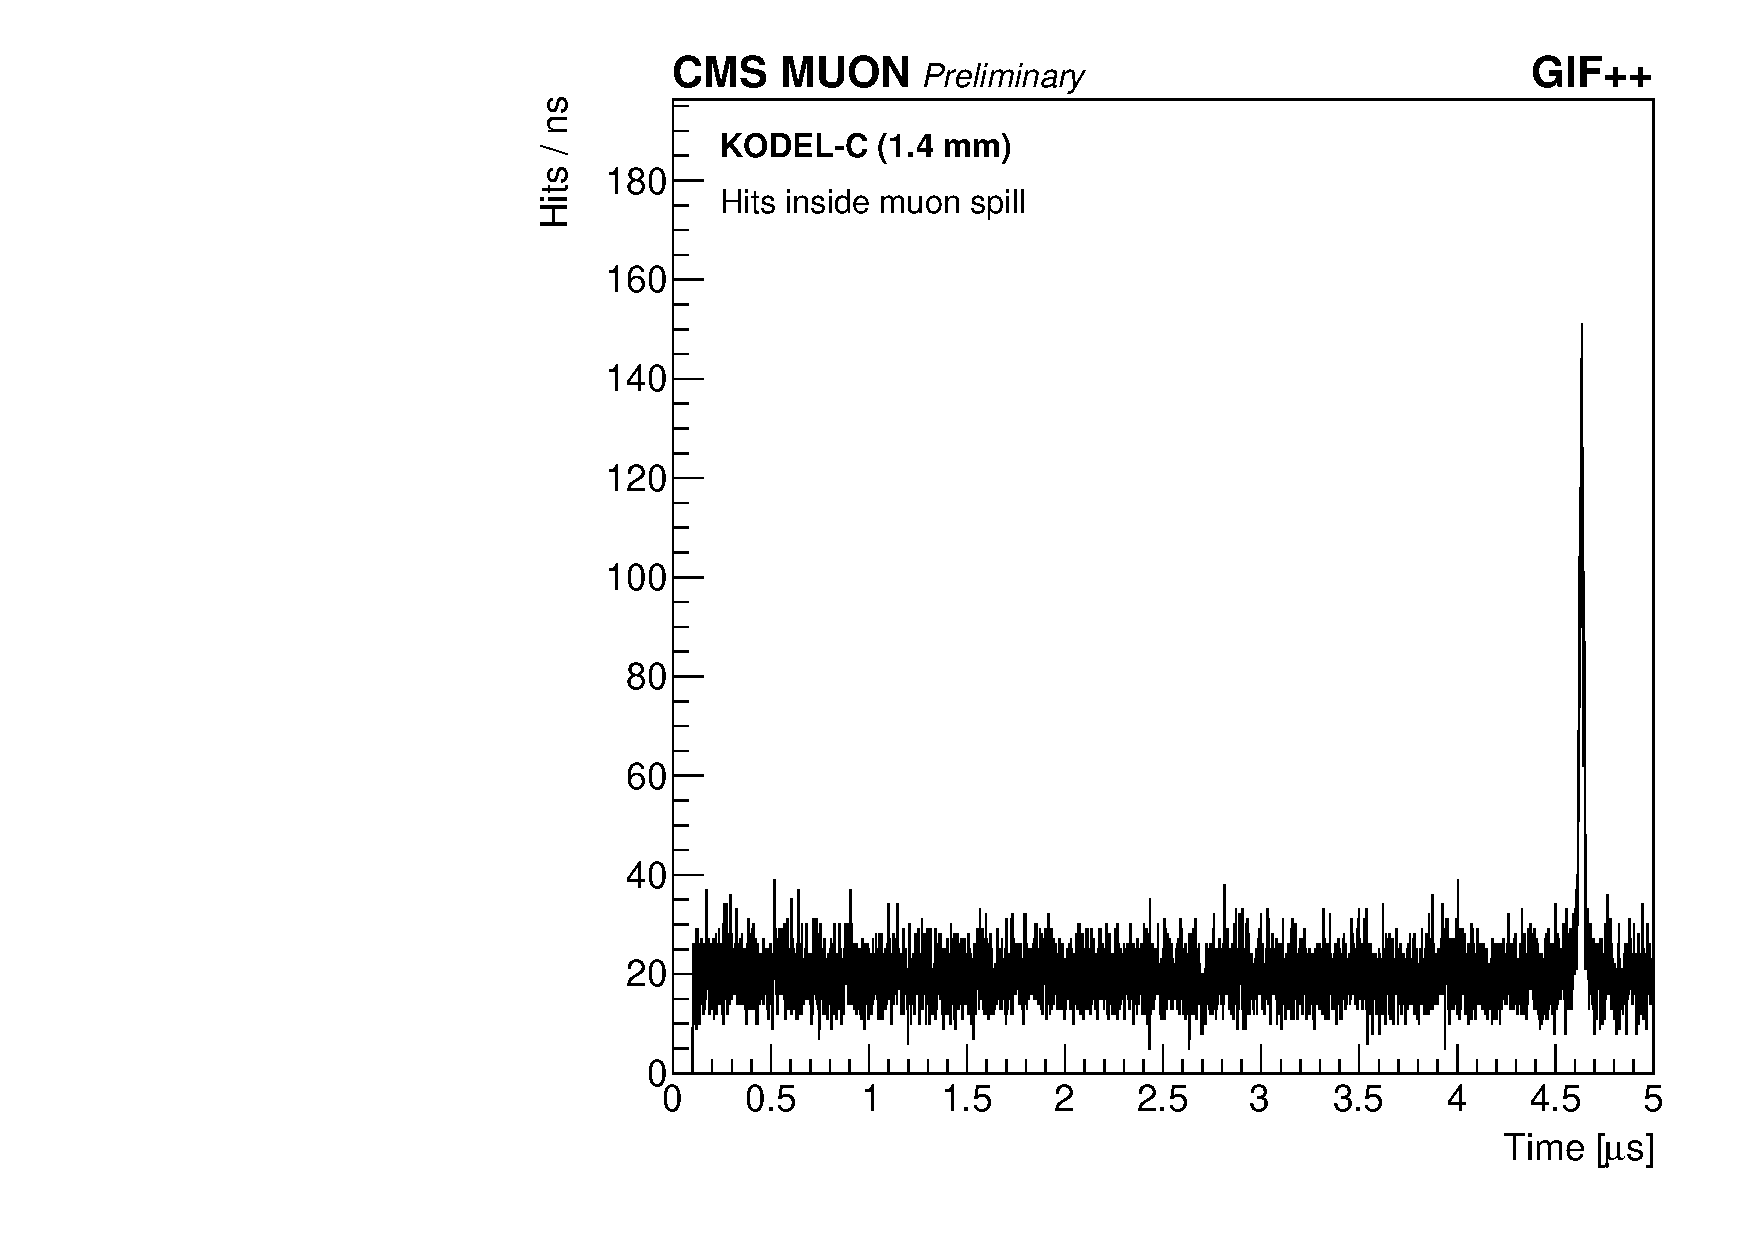
\includegraphics[width=0.45\textwidth]{figures/timeProfile_spill.pdf}}}\hfill
  \subfloat[][]{\label{subfig:RPC_hits_TDC_zoomed}%
    \fbox{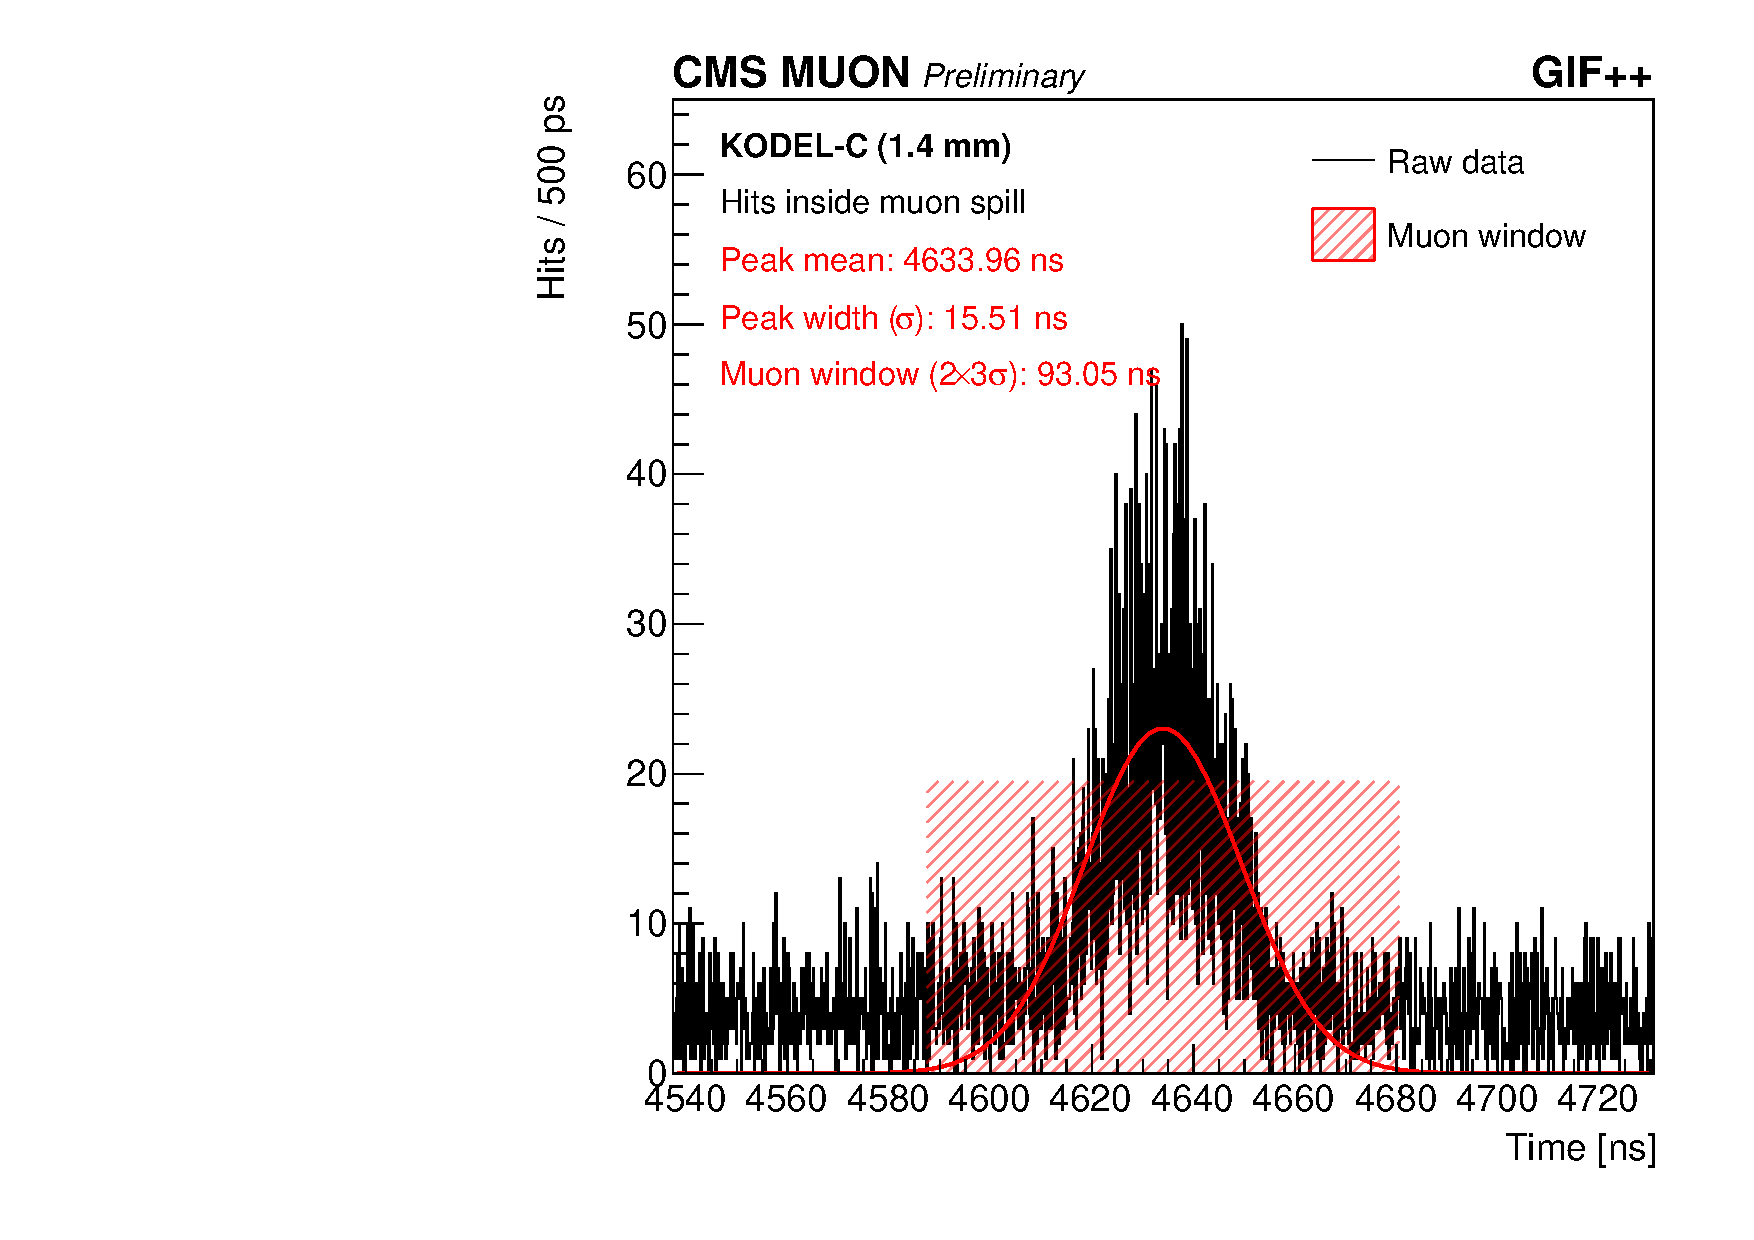
\includegraphics[width=0.45\textwidth]{figures/timeProfile_spill_zoomed.pdf}}}\\
  \legend{Hits recorded from a 1.4 mm double-gap chamber at GIF++. In (a) the is possible to see a narrow peak that comes from the triggered muon beam and a background that comes from gammas in (b) the time profile is zoomed in the muon beam region and a Gaussian fit is done to determine the muon time window.}
\end{figure}

The efficiency is calculated by 
\begin{equation}
    \epsilon_{tot} = N_{tot}/N_{evt},
\end{equation}
where the N$_{tot}$ are the number of events with at least 1 hit inside the muon time window and N$_{evt}$ is the number of recorded events. Still, this is have contamination of gammas that where detected inside the muon time window that. One strategy to remove the gamma contribution to the efficiency is to use the Bayes probability formula for dependent measurements
\begin{eqnarray}
    \epsilon_{tot} = \epsilon_\mu + \epsilon_\gamma - \epsilon_\mu \times \epsilon_\gamma, \nonumber \\ 
    \epsilon_\mu = \frac{\epsilon_{tot} - \epsilon_\gamma}{1-\epsilon_\gamma},
\end{eqnarray}
where $\epsilon_\gamma$ is the fake efficiency from gammas, that can be extracted by calculating the efficiency in a region outside of the muon window. and $\epsilon_\mu$ is the real muon efficiency. This approach was used to measure the muon efficiency for CMS RPC chambers during tests beams in 1997 at the old Gamma Irradiation Facility \cite{Layter:343814}. The gamma efficiency depends on the size of the time window, which is not optimal. Furthermore, for lower photon flux, the fake efficiency calculation can suffer from lower statistics. To have a more reliable efficiency measurements, the tracking system was proposed.

Figure \ref{fig:GIF_setup} shows the experimental setup at GIF++. There are two trolleys, in the one closest to the gamma source the test chamber is placed (from now on refereed to as KODEL-C). On the trolley farther from the gamma source, two tracking RPC chambers are installed (from now on refereed to as GT1 and GT2), with their strip planes oriented perpendicular to each other to allow measurement in two directions. Details on the used chambers characteristics.

\begin{figure}[!htm]{15cm}
\caption{Experimental Setup at GIF++.}%
\label{fig:GIF_setup}
\fbox{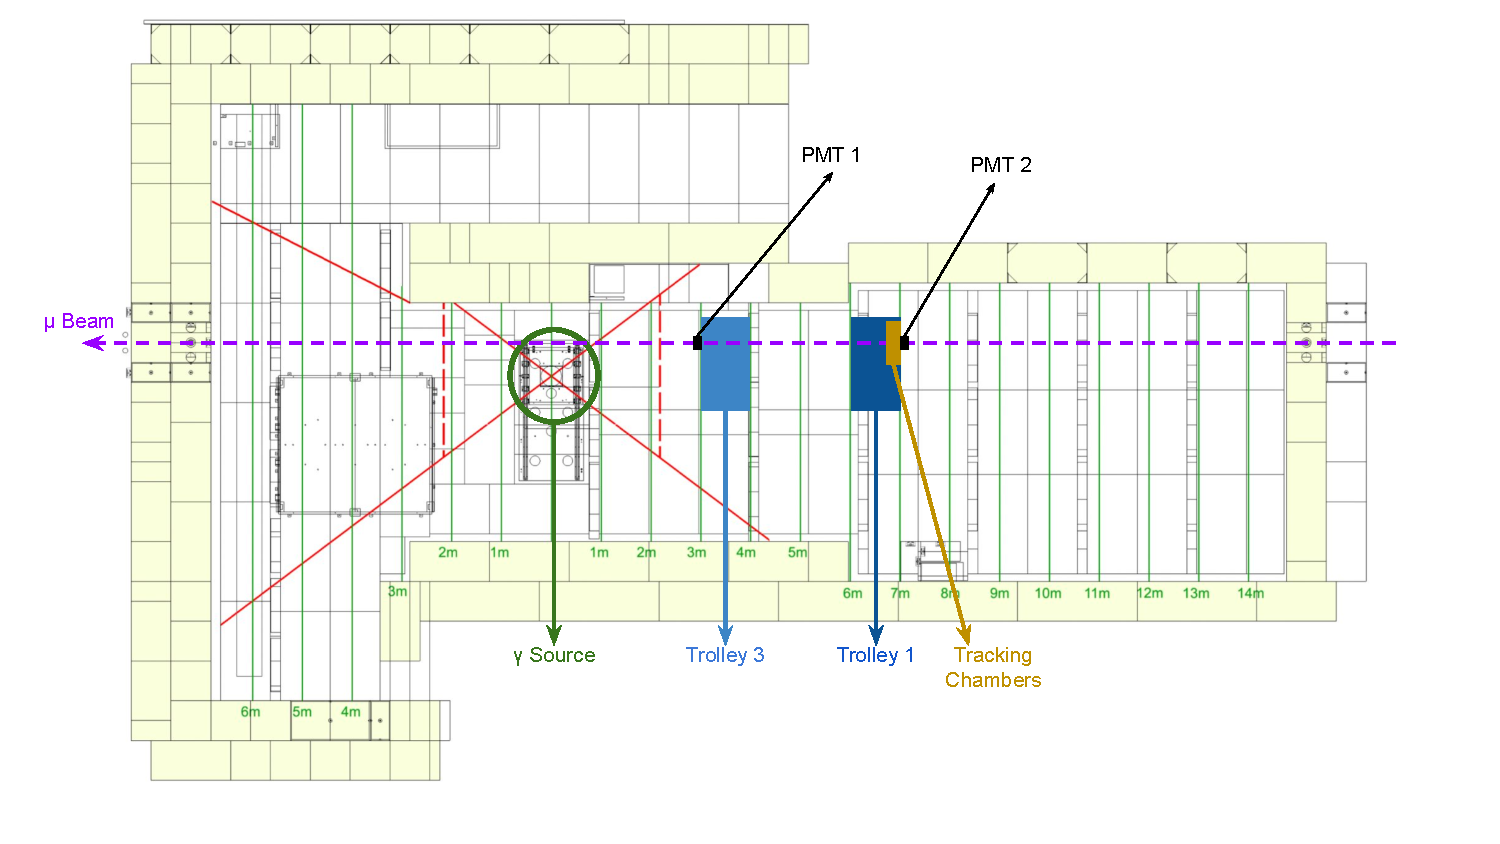
\includegraphics[width=0.7\hsize]{figures/GIF_setup.pdf}}
\legend{The experimental setup inside the GIF++ bunker. There are two trolleys where RPC chambers are placed for irradiation. The tracking chambers are located in the trolley farther from the gamma source.}
\source{\cite{https://doi.org/10.48550/arxiv.2211.16591}}
\end{figure}

\begin{table}[!htbp]{15cm}
\caption{Characteristics of the chambers used in the tracking analysis}\label{tab:RPCchar}
\begin{tabular}{|c|c|c|c|}
    \hline
    Name & Gap type & Strip Plane & Front-End Electronics \\
    \hline
    \multirow{2}{*}{GT1 (tracking)} & Double Gap HPL & 32 strips & CMS Electronics \\ 
     & 2mm thickness & 1.45 cm pitch & 150 fC, 100 ns port width \\
    \hline
    \multirow{2}{*}{GT2 (tracking)} & Double Gap HPL & 32 strips & CMS Electronics \\ 
     & 2mm thickness & 1.45 cm pitch & 150 fC, 100 ns port width \\
    \hline
    \multirow{2}{*}{KODEL-C (test)} & Double Gap HPL & 32 strips & Custom Electronics \\ 
     & 1.4mm thickness & 1.94 cm pitch & 75 fC, 60 ns port width \\
    \hline
\end{tabular}
\legend{Characteristics of the chambers used for the tracking and the test chamber to evaluate the performance of the algorithm}
\source{\cite{https://doi.org/10.48550/arxiv.2211.16591}}
\end{table}

To start the tracking analysis first the events are chosen so that at least there is at least one hit inside the muon time window for the two tracking chambers. This is required so that the the probability of hits from background or tracking is very low. A 2D hit profile is constructed to check the alignment of the tracking chambers and the muon beam (Fig. \ref{fig:2D_hit_profile}). the tracking chambers position in the trolley is adjusted so that the muon beam is centred in the run, this way we can avoid the muons to fall out of the detecting region by possible beam adjustments during the data taking. 

\begin{figure}[!htm]{15cm}
\caption{2D hit profile of tracking chambers at GIF++.}%
\label{fig:2D_hit_profile}
\fbox{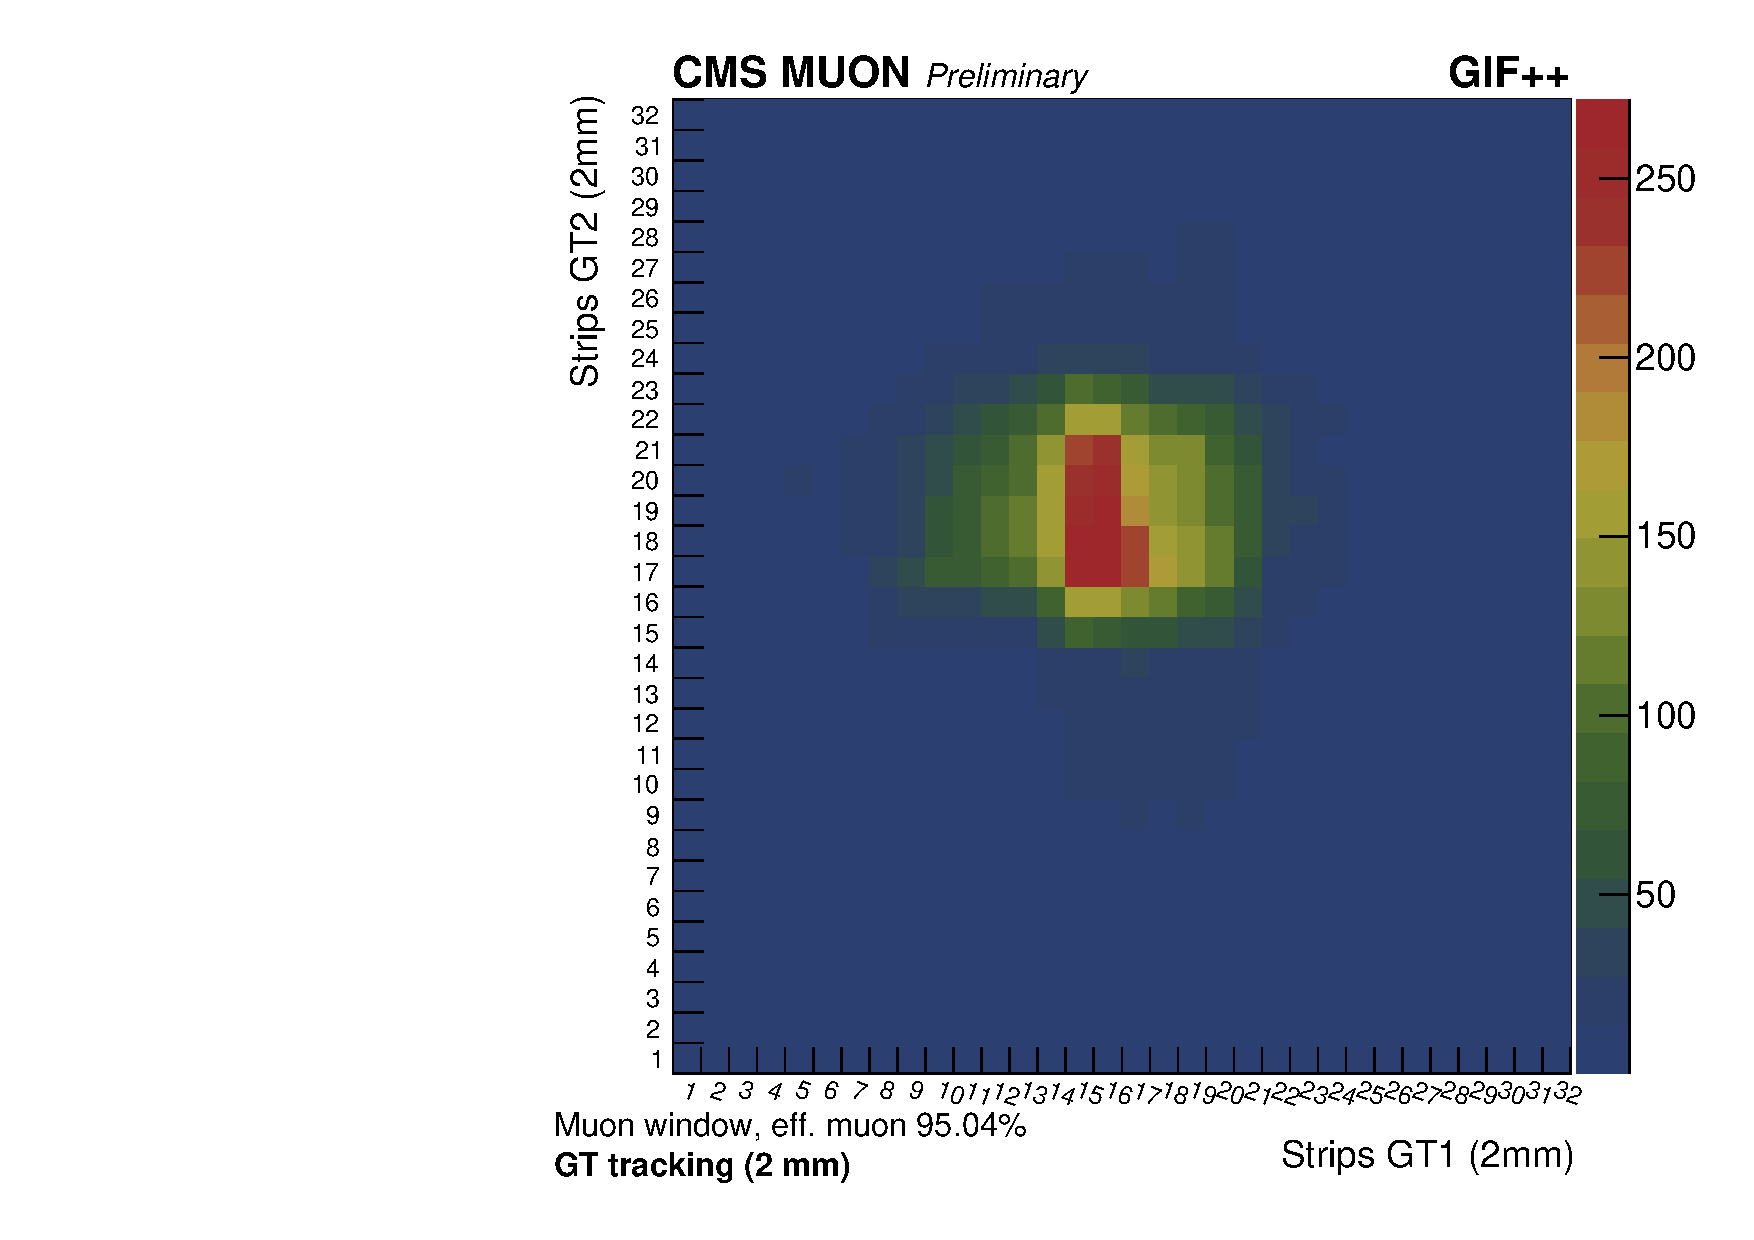
\includegraphics[width=0.7\hsize]{figures/muonHitProfile.pdf}}
\legend{2D hit profile from the tracking chambers at GIF++. The chambers' strip plane are oriented perpendicularly to each other so that it is possible to make a 2D hit mapping.}
\source{\cite{https://doi.org/10.48550/arxiv.2211.16591}}
\end{figure}

The tracking algorithm relies on the assumption that the beam is perpendicular to the strip plane, therefore it is only needed to extrapolate the position of the hit from the tracking to the test chamber and check for a matching hit. For every event, the following steps are taken \cite{https://doi.org/10.48550/arxiv.2211.16591}:
\begin{enumerate}
    \item Perform the clusterization of the hits in the tracking chambers, where events with more than one cluster are rejected. The cluster barycenters are defined as the mean position in the cluster;
    \item Perform the clusterization for the test chambers and calculate the clusters' barycenters;
    \item Form a perpendicular track starting from the tracking cluster barycenter;
    \item Check for a match in any cluster on the test chamber. 
\end{enumerate}

The clusterization is done by grouping hits that are adjacent and does not exceed a difference of time. The difference of time is previously determined in cosmic or source off data taking and depends on the chambers and front-end electronics and DAQ used. The cluster barycenter is defined as the geometrical mean position of the cluster. Figure \ref{fig:tracking_evt} shows an example of a event where a matching hit was found.

\begin{figure}[!htm]{15cm}
\caption{2D hit profile of tracking chambers at GIF++.}%
\label{fig:tracking_evt}
\fbox{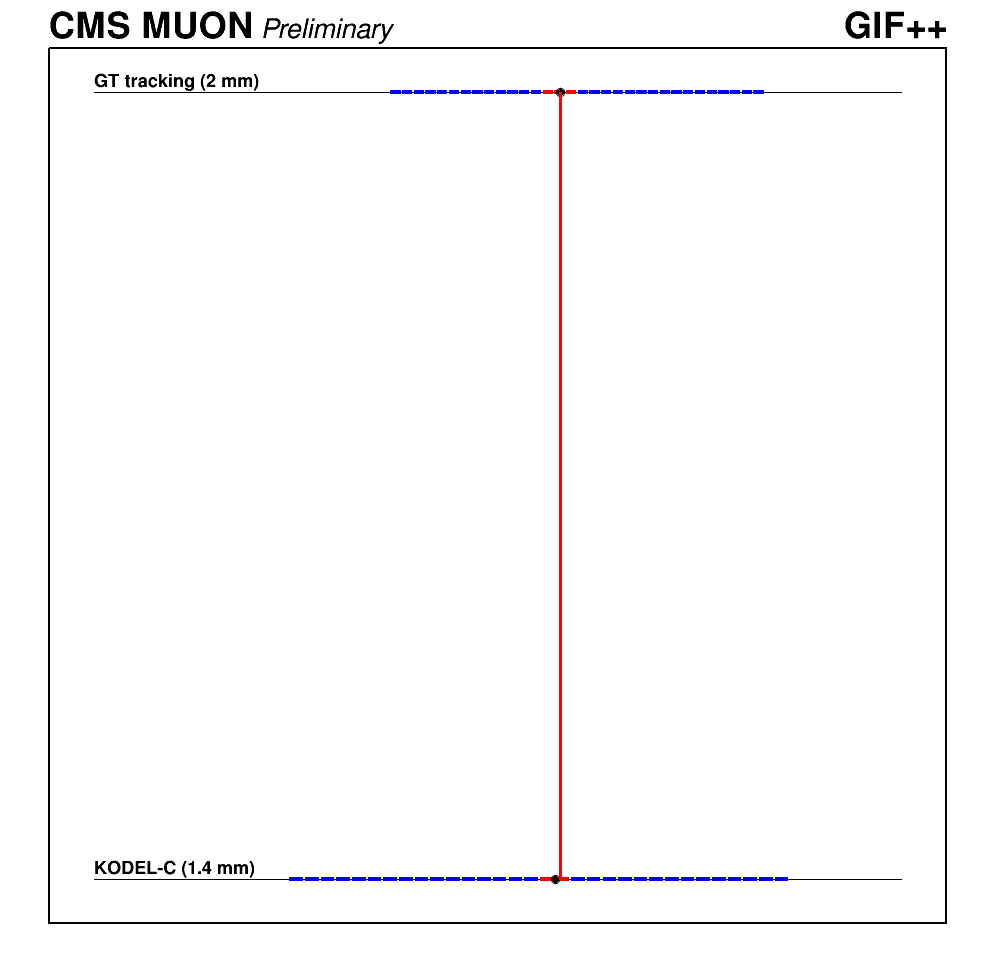
\includegraphics[width=0.5\hsize]{figures/event_0.png}}
\legend{Example of one event in which the hit on tracking chamber was matched on the test chamber. The strips in red represent the hits and the point in black is the 
cluster barycentre.}
\source{\cite{https://doi.org/10.48550/arxiv.2211.16591}}
\end{figure}

Efficiency curves of the test chambers were used to evaluate the validity of the tracking in rejecting the fake hits caused by the gammas. On Fig. \ref{fig:effcomparison} the efficiency curves are compared for three gamma background conditions. There are three curves in each plot. The black curve is calculated without the tracking, taking into consideration all the hits in the muon time window. For the blue one, only the hits that passed the tracking criteria were considered. Finally, for the red curve, the HV was recalculated to remove the voltage drop caused by the resistance of the electrodes using the Ohm law
\begin{equation}
    HV_{gas} = HV_{app} - R \cdot I,
\end{equation}
where HV$_gas$ is the corrected HV, HV$_{app}$ is the applied HV, R is the resistance of the electrode, determined previously by argon scans \cite{peskov2018resistive}. This correction decouples the shift to the right of the curve on higher cluster rates, caused by the increase of the current. Therefore, HV$_{gas}$ is the effective HV applied to the gas volume. 

\begin{figure}[!htm]{15cm}
  \caption{Comparison of the tracking algorithm using efficiency curves.} 
  \label{fig:effcomparison}
  \subfloat[][]{\label{subfig:ABSOFF}%
    \fbox{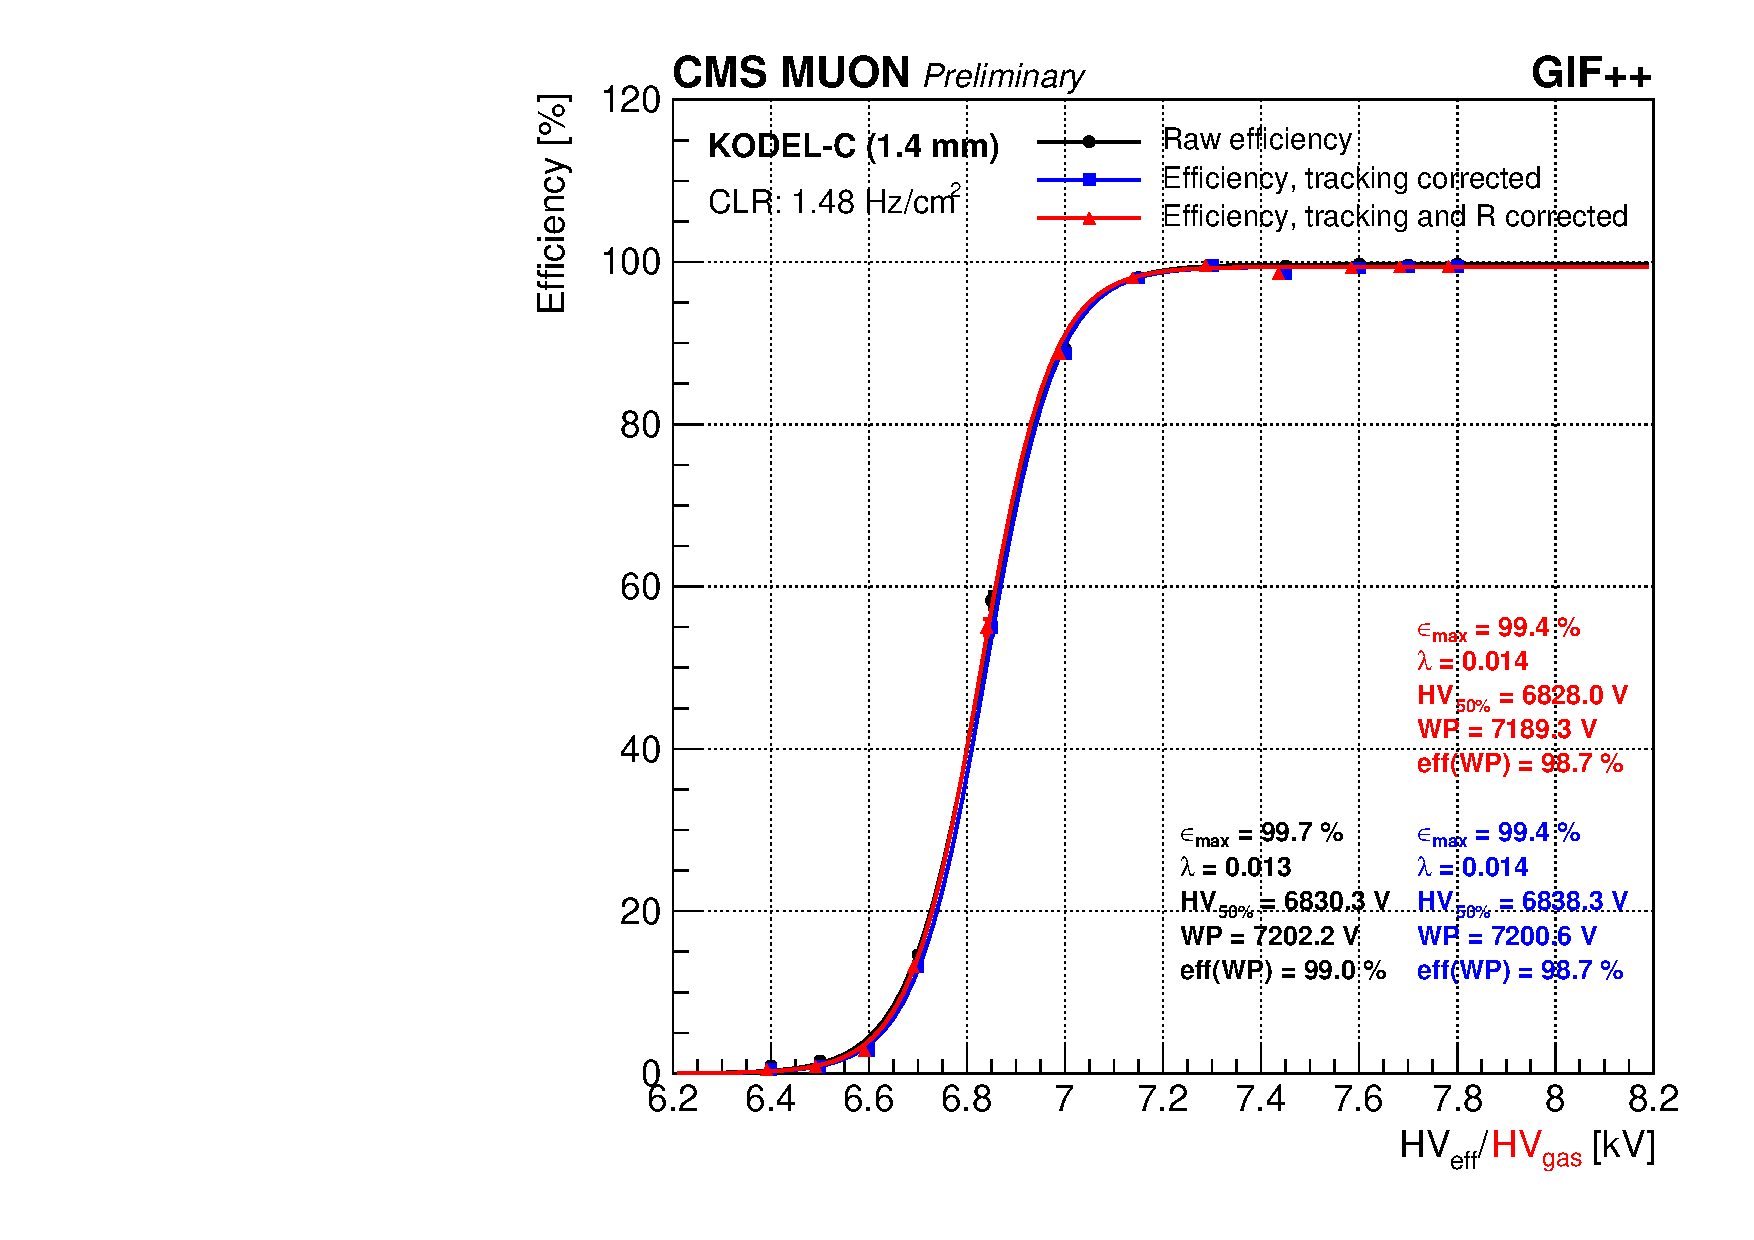
\includegraphics[width=0.45\textwidth]{figures/all_ABS_OFF.pdf}}}\hfill
  \subfloat[][]{\label{subfig:ABS10}%
    \fbox{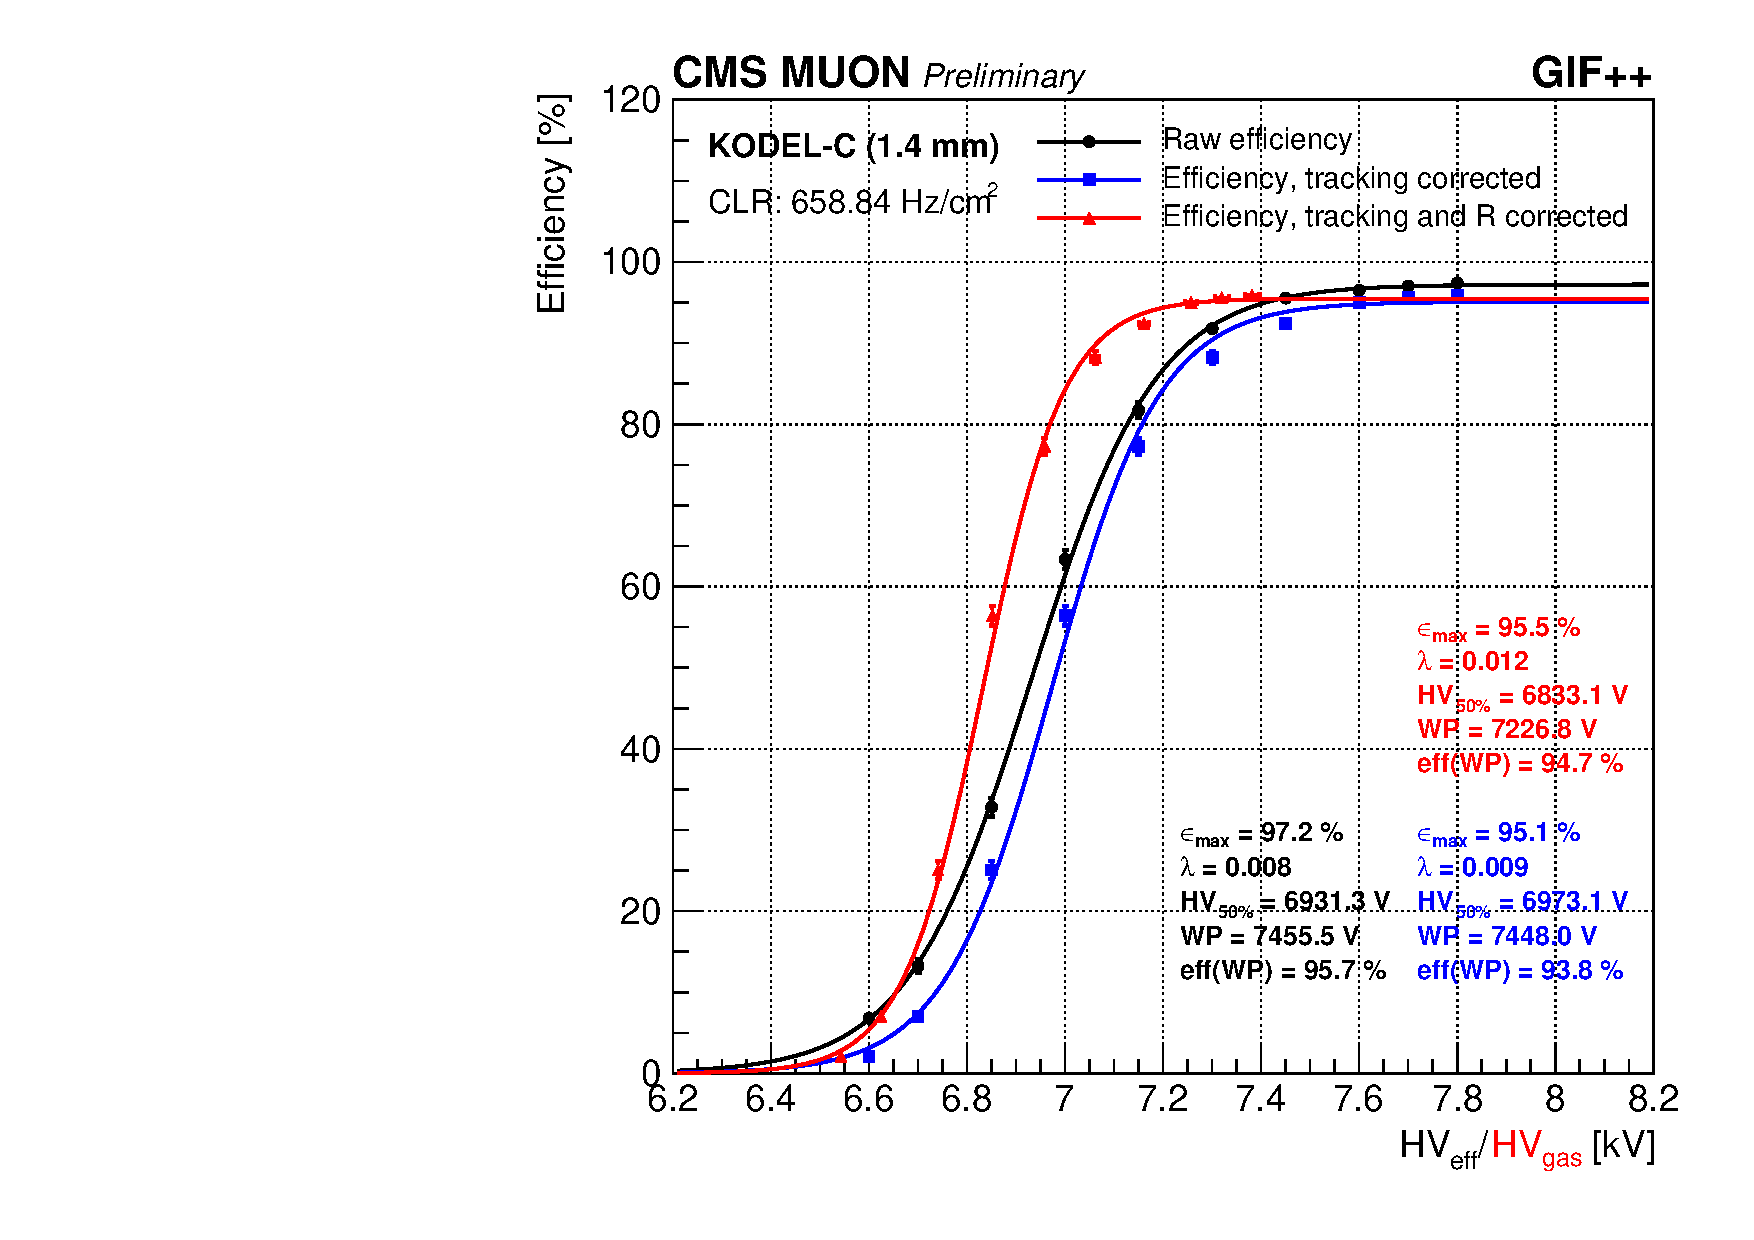
\includegraphics[width=0.45\textwidth]{figures/all_ABS_10.pdf}}}
    \hfill
  \subfloat[][]{\label{subfig:ABS3p3}%
    \fbox{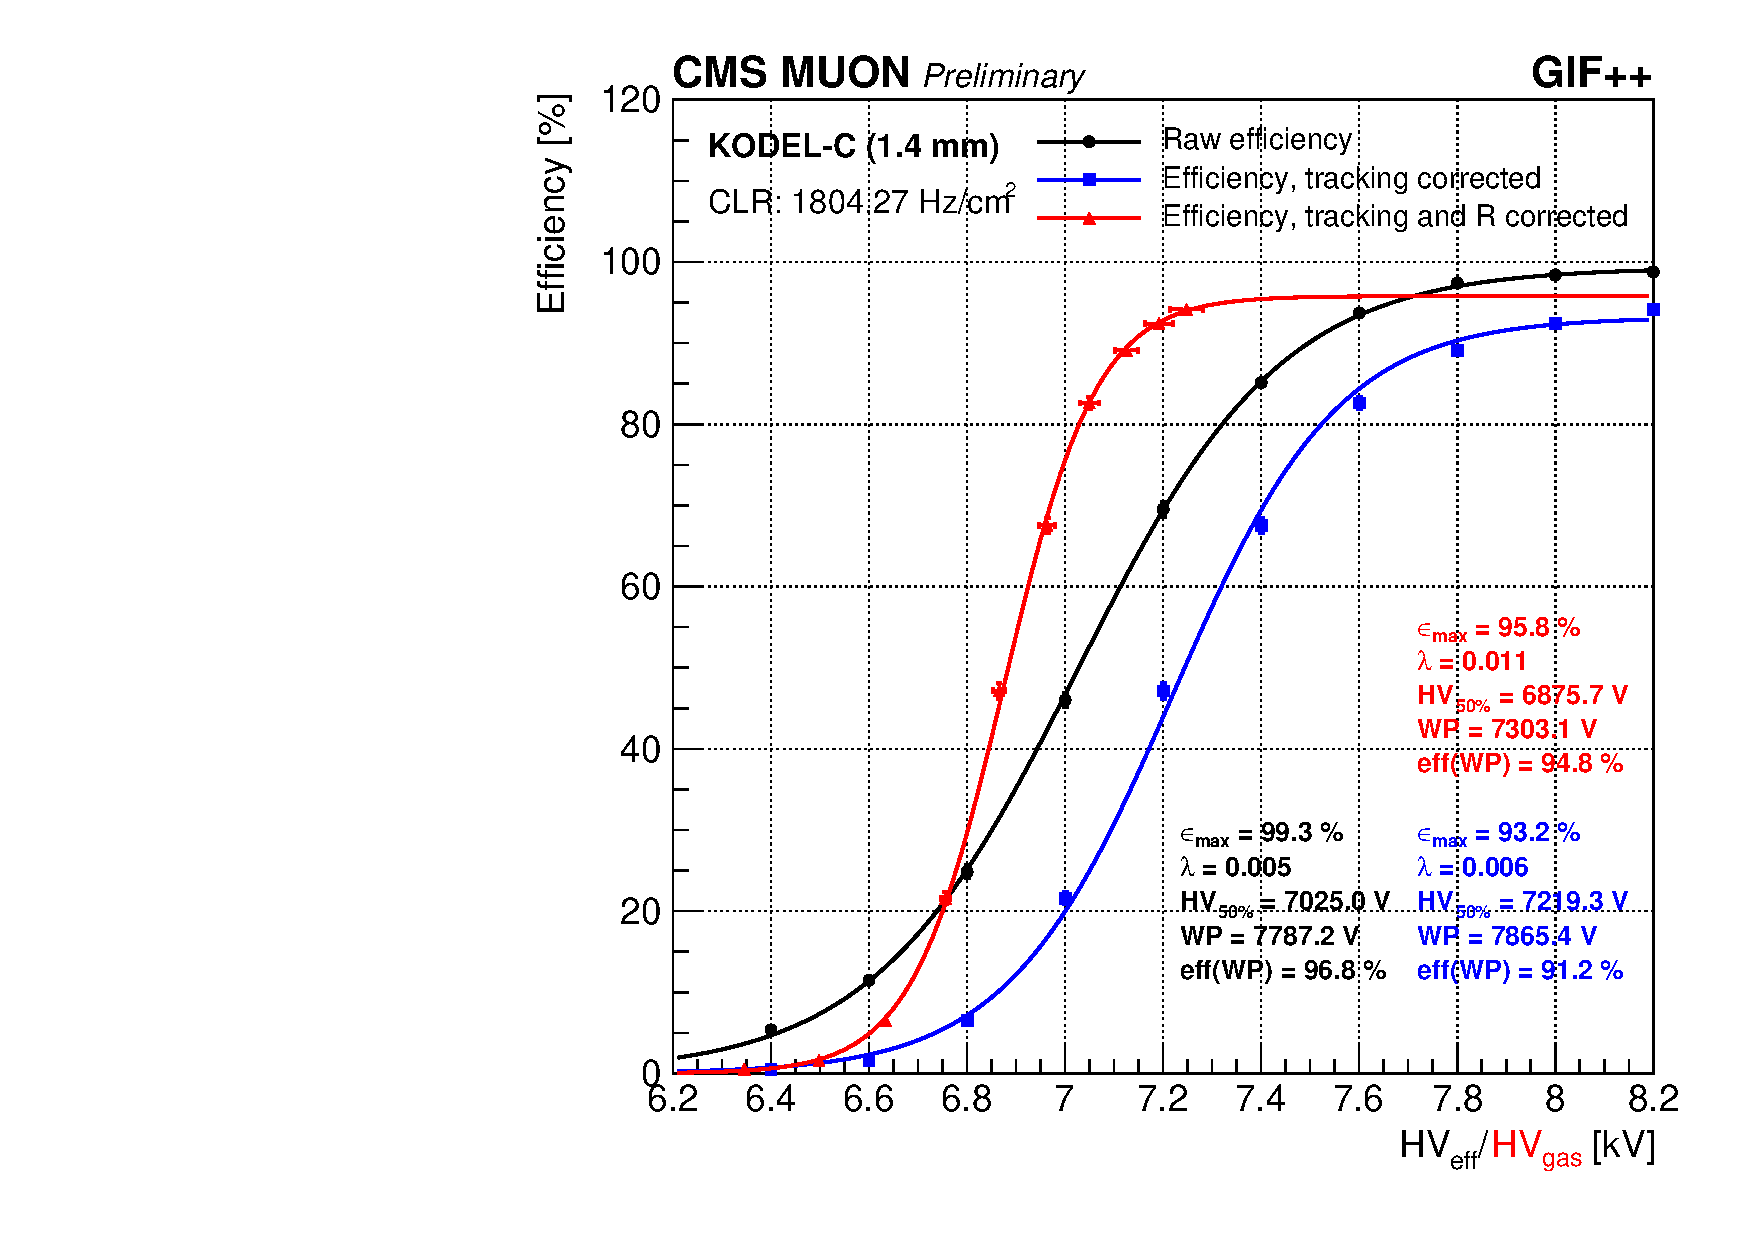
\includegraphics[width=0.45\textwidth]{figures/all_ABS_3p3.pdf}}}\\
  \legend{Efficiencies and their sigmoid fits measured at three photon fluxes with measured at the working-point high voltages gamma cluster rates of 1.804 kHz (a), 0.645 kHz (b), and 1.48 Hz (c), respectively. The curve in black is the efficiency calculated with all hits inside the muon window, the blue one is with applied tracking correction and the one in red -- with tracking and resistance correction.}
  \source{\cite{https://doi.org/10.48550/arxiv.2211.16591}}
\end{figure}

In Fig. \ref{subfig:ABSOFF} the curves are equivalent, this behavior is expected, since at lower rates, the currents are low, so there are no fake hits nor HV correction. In Figure \ref{subfig:ABS10}, the background rate becomes substantial, so we can see a shift to the right in the curves without resistance correction, caused by the aforementioned voltage drop, which is much more noticeable in Fig. \ref{subfig:ABS10}. A decrease of the maximum efficiency with the increase of rate is expected, because of the dead time of the front-end electronics, but we can see an increase in the raw efficiency, which indicates a high fake hit contamination.

To finalize the discussion, the plots of the efficiency curves with tracking and with tracking and resistance correction can be seen in Fig. \ref{fig:eff_curves}. The effect of the voltage drop on the electrodes is very noticeable in Fig. \ref{subfig:sigmoids_trk} and it is also possible to see the expected decrease maximum efficiency, proving that the fake hit contamination was removed using the tracking. In Fig. \ref{subfig:sigmoids_trk_corr} it is still possible to see a shift to the right in the curves, this is also expected, since the high rates induce an efficiency drop in the RPCs, because of the reduce of the gas amplification caused by the space charge effect \cite{Lippmann:2003yb}. 

\begin{figure}[!htm]{15cm}
  \caption{Efficiency curves for various gamma background rates.} 
  \label{fig:eff_curves}
  \subfloat[][]{\label{subfig:sigmoids_trk}%
    \fbox{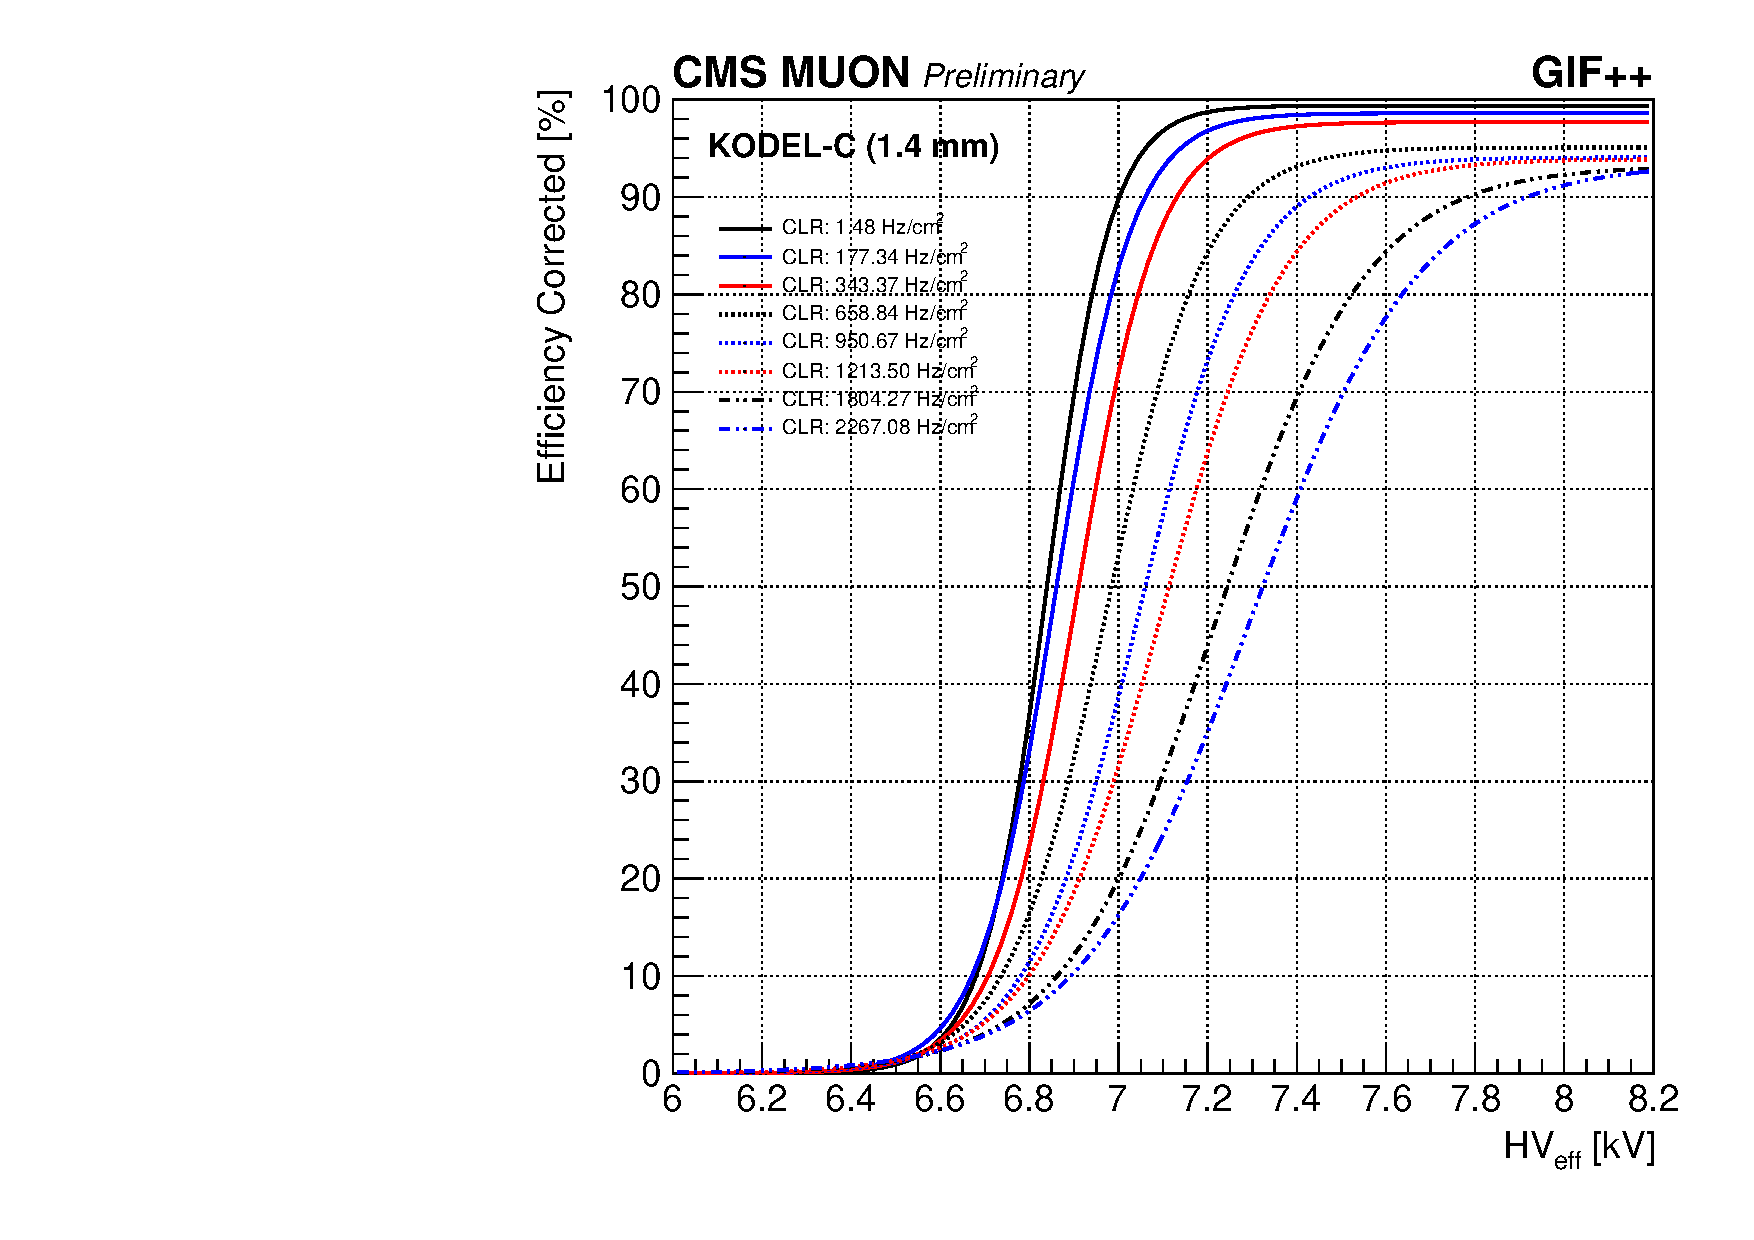
\includegraphics[width=0.45\textwidth]{figures/sigmoids_trk.pdf}}}\hfill
  \subfloat[][]{\label{subfig:sigmoids_trk_corr}%
    \fbox{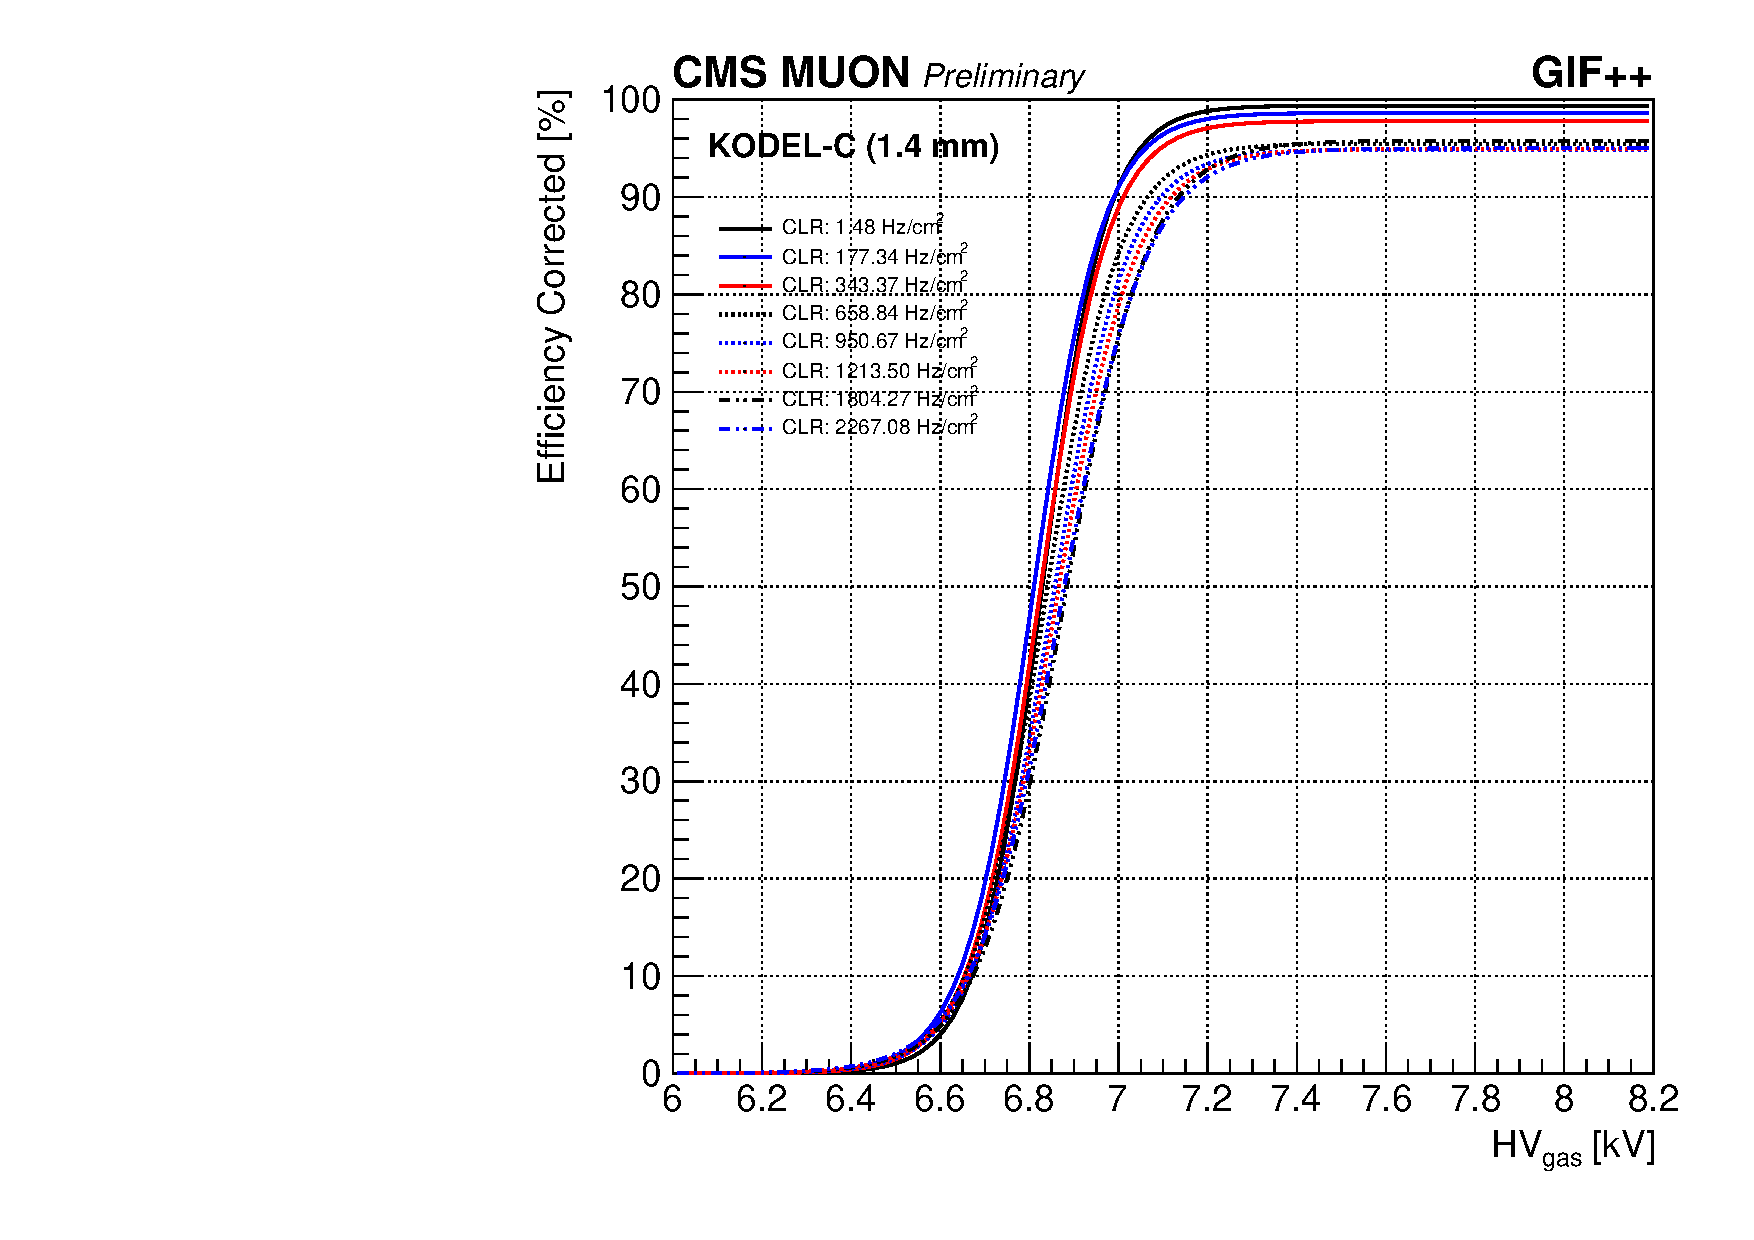
\includegraphics[width=0.45\textwidth]{figures/sigmoids_trk_corr.pdf}}}\\
  \legend{Efficiency curves for various gamma background rates. In (a) the HV applied is corrected only by pressure and temperature (HV$_{eff}$), while in (b) the HV is also corrected by the resistance of the gaps (HV$_{gas}$).}
  \source{\cite{https://doi.org/10.48550/arxiv.2211.16591}}
\end{figure}

The tracking system implementation at GIF++ was successful, and was able to remove the fake hit contribution. The KODEL-C is a prototype used to evaluate the performance of the 1.4 mm gaps, the same used in the iRPC design. It showed good results in the high rate environment, even at rates higher than 2 kHz/cm$^2$, with increase on the working point of $\approx$650 V with efficiency loss of $\approx$ 7.5\%, using a custom front-end. The iRPC front-end design have lower threshold and dead time so it is expected to perform better \cite{CMS:2021bxv}.